\section{Results}

\subsection{rajat12}
\begin{figure}
\centering
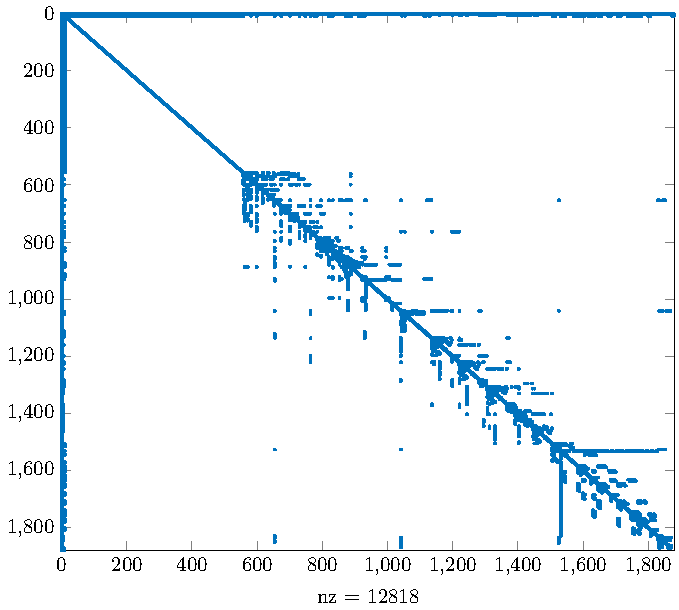
\includegraphics[scale=0.8]{../src/figure/rajat12.pdf}
\caption{Sparsity representation of the \texttt{rajat12} matrix.}
\label{fig:rajat12}
\end{figure}
Figure~\ref{fig:rajat12} shows the \texttt{rajat12} circuit matrix. This matrix is real and the matlab routine \texttt{issymmetric} finds it to be not symmetric. From a complex point of view it can thus be considered non-hermitian. However a closer look at Figure~\ref{fig:rajat12} reveals that the matrix is very close to being symmetric. In a first series of experiments the iterative GMRES method is used. The level of the incomplete LU-factorization, which is used for preconditioning is varied from between zero and one. Furthermore the amount of available vectors is increased successively from zero to one hundred. \\
Results for the time measurements are shown in figure~\ref{fig:iluRajatCompTime}. The data shows a significant increase in computation time, for higher numbers of available vectors, with a zero level of fill. The same observation does not hold with a level of fill of one, here computations oscillate around an expected value of approximately two seconds. \\
Figure~\ref{fig:rajatConvergence} shows convergence of the residual using 10 Vectors with zero level of fill in blue and level of fill 1 in red. Here it is important to note, that sufficient accuracy is reached using 10 Vectors within $\approx 230$ iterations for ILU level zero. It takes $\approx 20$ when the level of fill is set to one. Curiously the decrease in iterations not lead to on overall reduction of computation time. Probably in this case single iterations are much faster with zero level of fill, which would account for the timing difference. An overall increase of computations time can be observed for more vectors with in the zero level of fill setting. This is probably due to the fact that the overhead caused by the additional vectors becomes significant only when the amount of total iterations is large. Interestingly, when more vectors are used fewer iterations are required until convergence is reached. Large amounts of vectors are probably beneficial in settings, where larger matrices are used.
Memory requirements are shown in table~\ref{tab:RajatMemoryGMRES}. From the date it can be concluded that the higher ilu level does is neither 
advantageous in terms of memory consumption or computing time when the relatively small circuit matrix is considered. \\
Figure~\ref{fig:rajatSpectra}, shows the initial and preconditioned spectra. The normalizing effect of both preconditioners is clearly visible. Following the rule of thumb\footnote{Numerical linear algebra, Trefethen, Bau, page 314}: \\
\textquotedblleft A preconditioner $M$ is good if $M^{-1}$A is not too far from normal and its eigenvalues are clustered.\textquotedblright \\
Both preconditioners work but the higher level of fill gives more clustering, therefore it is better in this case.
The direct method implemented in the \texttt{mumps} requires \texttt{5.08 MB}  of ram and finishes within $0.004035s = 4.035*10^{-3}s$. It is thus faster then any iterative scheme tried above, with more then acceptable memory consumption. Storing some data on the hard drive using the \texttt{--ooc} option increases the computation time to $0.007442s$. In this cases this is clearly not necessary, as the memory needed is available on almost any modern computer.

\begin{figure}
\centering
% This file was created by matlab2tikz.
% Minimal pgfplots version: 1.3
%
%The latest updates can be retrieved from
%  http://www.mathworks.com/matlabcentral/fileexchange/22022-matlab2tikz
%where you can also make suggestions and rate matlab2tikz.
%
\documentclass[tikz]{standalone}
\usepackage{pgfplots}
\usepackage{grffile}
\pgfplotsset{compat=newest}
\usetikzlibrary{plotmarks}
\usepackage{amsmath}

\begin{document}
\definecolor{mycolor1}{rgb}{0.00000,0.44700,0.74100}%
%
\begin{tikzpicture}

\begin{axis}[%
width=1.5in,
height=1.5in,
at={(1.658854in,0.483542in)},
scale only axis,
xmin=0,
xmax=100,
xlabel={vectors},
ymin=0.016,
ymax=0.034,
ylabel={time [s]}
]
\addplot [color=mycolor1,solid,forget plot]
  table[row sep=crcr]{%
10	0.018125\\
11	0.022677\\
12	0.019412\\
13	0.020491\\
14	0.020396\\
15	0.019024\\
16	0.018773\\
17	0.017667\\
18	0.018628\\
19	0.017929\\
20	0.018139\\
21	0.018121\\
22	0.017523\\
23	0.019255\\
24	0.018598\\
25	0.018323\\
26	0.018326\\
27	0.018363\\
28	0.018373\\
29	0.01925\\
30	0.018653\\
31	0.01873\\
32	0.019364\\
33	0.019391\\
34	0.019466\\
35	0.019565\\
36	0.019688\\
37	0.019458\\
38	0.019964\\
39	0.020066\\
40	0.020697\\
41	0.021627\\
42	0.021546\\
43	0.020978\\
44	0.021024\\
45	0.021487\\
46	0.021248\\
47	0.021167\\
48	0.021313\\
49	0.021178\\
50	0.020938\\
51	0.021249\\
52	0.021826\\
53	0.022879\\
54	0.022944\\
55	0.023355\\
56	0.024061\\
57	0.024749\\
58	0.026311\\
59	0.025305\\
60	0.026383\\
61	0.026179\\
62	0.026303\\
63	0.027102\\
64	0.027013\\
65	0.025844\\
66	0.02657\\
67	0.026707\\
68	0.026278\\
69	0.025464\\
70	0.026814\\
71	0.025882\\
72	0.026522\\
73	0.025867\\
74	0.026382\\
75	0.026203\\
76	0.026442\\
77	0.026184\\
78	0.027455\\
79	0.027266\\
80	0.026837\\
81	0.028027\\
82	0.027961\\
83	0.027959\\
84	0.0292\\
85	0.028966\\
86	0.028973\\
87	0.029637\\
88	0.029366\\
89	0.030741\\
90	0.033256\\
91	0.030473\\
92	0.03094\\
93	0.032107\\
94	0.032836\\
95	0.032143\\
96	0.031817\\
97	0.032091\\
98	0.032285\\
99	0.033414\\
100	0.032784\\
};
\end{axis}

\begin{axis}[%
width=1.5in,
height=1.5in,
at={(4in,0.483542in)},
scale only axis,
xmin=0,
xmax=100,
xlabel={vectors},
ymin=1.6,
ymax=2.4,
ylabel={time [s]}
]
\addplot [color=mycolor1,solid,forget plot]
  table[row sep=crcr]{%
10	1.74676\\
11	1.71041\\
12	1.70631\\
13	1.70142\\
14	1.75954\\
15	1.84593\\
16	1.6833\\
17	1.70468\\
18	1.82023\\
19	1.76165\\
20	1.88569\\
21	1.77032\\
22	1.96255\\
23	1.74319\\
24	1.75664\\
25	2.108\\
26	1.82673\\
27	1.77709\\
28	1.70632\\
29	1.95466\\
30	1.76682\\
31	1.74808\\
32	1.75602\\
33	1.71269\\
34	1.7341\\
35	1.93888\\
36	1.75801\\
37	1.82413\\
38	1.83235\\
39	1.69602\\
40	1.72439\\
41	1.76215\\
42	1.72729\\
43	1.739\\
44	1.69348\\
45	1.84948\\
46	1.69432\\
47	1.71769\\
48	1.89903\\
49	1.77071\\
50	1.99037\\
51	1.67983\\
52	1.83828\\
53	1.92141\\
54	2.01674\\
55	1.80825\\
56	1.79346\\
57	1.86234\\
58	1.76435\\
59	1.74363\\
60	1.70756\\
61	1.71482\\
62	1.87778\\
63	1.69935\\
64	1.78105\\
65	1.7007\\
66	2.11195\\
67	1.7423\\
68	1.98093\\
69	1.84952\\
70	1.71318\\
71	2.0918\\
72	2.2592\\
73	2.24579\\
74	2.11869\\
75	2.21775\\
76	1.97425\\
77	2.35217\\
78	1.74441\\
79	1.71436\\
80	1.71036\\
81	2.08705\\
82	1.68541\\
83	1.76413\\
84	1.69961\\
85	1.69041\\
86	1.68632\\
87	1.68961\\
88	1.68019\\
89	1.67906\\
90	1.68073\\
91	1.68\\
92	1.69037\\
93	1.69836\\
94	1.6879\\
95	1.86636\\
96	1.7987\\
97	1.7434\\
98	1.79029\\
99	1.82523\\
100	1.72024\\
};
\end{axis}
\end{tikzpicture}%
\end{document}
\caption{CPU-Time of running \texttt{./ilu --method gmres --file rajat12.mtx  --nvectors \$vectors --tolerance 1.e-10} with \texttt{--ilu-level 0}(left) and \texttt{--ilu-level 1}(right) the value of the \texttt{\$vectors} variable is shown on the x axis.}
\label{fig:iluRajatCompTime}
\end{figure} 
\begin{figure}
\centering
% This file was created by matlab2tikz.
% Minimal pgfplots version: 1.3
%
%The latest updates can be retrieved from
%  http://www.mathworks.com/matlabcentral/fileexchange/22022-matlab2tikz
%where you can also make suggestions and rate matlab2tikz.
%
\documentclass[tikz]{standalone}
\usepackage{pgfplots}
\usepackage{grffile}
\pgfplotsset{compat=newest}
\usetikzlibrary{plotmarks}
\usepackage{amsmath}

\begin{document}
\definecolor{mycolor1}{rgb}{0.00000,0.44700,0.74100}%
\definecolor{mycolor2}{rgb}{0.85000,0.32500,0.09800}%
%
\begin{tikzpicture}

\begin{axis}[%
width=2in,
height=2in,
at={(0.771875in,0.483542in)},
scale only axis,
xmin=0.197285105599905,
xmax=11.1661763577663,
ymin=-3.30394745235974,
ymax=525.599570869926
]
\addplot [color=mycolor1,solid,line width=2.0pt,forget plot]
  table[row sep=crcr]{%
1	500.369\\
2	22.038\\
3	19.6888\\
4	15.3888\\
5	3.80827\\
6	3.47815\\
7	2.38605\\
8	1.67397\\
9	0.881279\\
10	0.764443\\
11	0.63658\\
12	0.63595\\
13	0.617115\\
14	0.561676\\
15	0.49268\\
16	0.441212\\
17	0.314882\\
18	0.3014\\
19	0.250091\\
20	0.20548\\
21	0.189347\\
22	0.188932\\
23	0.188922\\
24	0.165311\\
25	0.139327\\
26	0.119566\\
27	0.111493\\
28	0.104409\\
29	0.0956074\\
30	0.0818959\\
31	0.0746758\\
32	0.074504\\
33	0.0738679\\
34	0.0657146\\
35	0.0585845\\
36	0.0555147\\
37	0.0459553\\
38	0.0399038\\
39	0.038795\\
40	0.0352988\\
41	0.0280612\\
42	0.0280388\\
43	0.0280038\\
44	0.0229191\\
45	0.0223529\\
46	0.0217129\\
47	0.0196485\\
48	0.0192655\\
49	0.0163879\\
50	0.015491\\
51	0.0151046\\
52	0.0148836\\
53	0.0148294\\
54	0.0140856\\
55	0.0126093\\
56	0.0119374\\
57	0.0109909\\
58	0.0108273\\
59	0.0107408\\
60	0.00786344\\
61	0.0074886\\
62	0.00748795\\
63	0.00743965\\
64	0.00626089\\
65	0.00621341\\
66	0.00596183\\
67	0.00522652\\
68	0.00517355\\
69	0.00492205\\
70	0.00433876\\
71	0.00421775\\
72	0.00421633\\
73	0.00418939\\
74	0.00405748\\
75	0.00380341\\
76	0.0035799\\
77	0.00335351\\
78	0.00314137\\
79	0.00298536\\
80	0.00259294\\
81	0.00196418\\
82	0.00196293\\
83	0.00192117\\
84	0.0015099\\
85	0.00142025\\
86	0.00136509\\
87	0.00117798\\
88	0.00113713\\
89	0.0010902\\
90	0.00105662\\
91	0.00101922\\
92	0.00101528\\
93	0.00101238\\
94	0.00094254\\
95	0.000915138\\
96	0.000817576\\
97	0.00077624\\
98	0.000699672\\
99	0.00069922\\
100	0.000502859\\
101	0.000395298\\
102	0.000395094\\
103	0.00039069\\
104	0.000327492\\
105	0.000280976\\
106	0.000228794\\
107	0.000209661\\
108	0.000208141\\
109	0.000186724\\
110	0.000173392\\
111	0.0001627\\
112	0.000161835\\
113	0.000160896\\
114	0.000158127\\
115	0.000147882\\
116	0.000143068\\
117	0.000120373\\
118	0.000116713\\
119	0.000103079\\
120	8.80536e-05\\
121	7.24922e-05\\
122	7.24826e-05\\
123	7.05322e-05\\
124	6.62605e-05\\
125	5.13077e-05\\
126	4.37749e-05\\
127	4.3153e-05\\
128	3.71366e-05\\
129	3.56918e-05\\
130	3.44443e-05\\
131	3.33401e-05\\
132	3.33114e-05\\
133	3.33114e-05\\
134	3.22308e-05\\
135	3.09106e-05\\
136	2.94616e-05\\
137	2.63044e-05\\
138	2.42314e-05\\
139	2.10179e-05\\
140	1.97969e-05\\
141	1.41261e-05\\
142	1.41059e-05\\
143	1.20928e-05\\
144	9.707e-06\\
145	8.81524e-06\\
146	7.52536e-06\\
147	7.45899e-06\\
148	6.99572e-06\\
149	6.51222e-06\\
150	6.40995e-06\\
151	6.23656e-06\\
152	6.2344e-06\\
153	6.2106e-06\\
154	5.98066e-06\\
155	5.84211e-06\\
156	5.7219e-06\\
157	5.05238e-06\\
158	4.75099e-06\\
159	3.92556e-06\\
160	3.73283e-06\\
161	3.38453e-06\\
162	3.37949e-06\\
163	3.30204e-06\\
164	2.92418e-06\\
165	2.56884e-06\\
166	2.31386e-06\\
167	2.1542e-06\\
168	2.02591e-06\\
169	2.01431e-06\\
170	1.89075e-06\\
171	1.66982e-06\\
172	1.66969e-06\\
173	1.62946e-06\\
174	1.48291e-06\\
175	1.44125e-06\\
176	1.39392e-06\\
177	1.3457e-06\\
178	1.32349e-06\\
179	1.19676e-06\\
180	1.17721e-06\\
181	1.01229e-06\\
182	1.01007e-06\\
183	1.00896e-06\\
184	9.12563e-07\\
185	8.56499e-07\\
186	8.26235e-07\\
187	7.55695e-07\\
188	7.36479e-07\\
189	7.05934e-07\\
190	6.75887e-07\\
191	6.69514e-07\\
192	6.68901e-07\\
193	6.65051e-07\\
194	6.28447e-07\\
195	5.9542e-07\\
196	5.76106e-07\\
197	5.34408e-07\\
198	5.20654e-07\\
199	4.81141e-07\\
200	4.51509e-07\\
201	3.92349e-07\\
202	3.92214e-07\\
203	3.59065e-07\\
204	3.28527e-07\\
205	3.03682e-07\\
206	2.99775e-07\\
207	2.59004e-07\\
208	2.55535e-07\\
209	2.55182e-07\\
210	2.37036e-07\\
211	2.33896e-07\\
212	2.33864e-07\\
213	2.33286e-07\\
214	2.22686e-07\\
215	2.17212e-07\\
216	2.04802e-07\\
217	1.8963e-07\\
218	1.82018e-07\\
219	1.67664e-07\\
220	1.55414e-07\\
221	1.49292e-07\\
222	1.49091e-07\\
223	1.42232e-07\\
224	1.28799e-07\\
225	1.22304e-07\\
226	1.10614e-07\\
227	1.10423e-07\\
228	9.92083e-08\\
229	9.77978e-08\\
230	9.63762e-08\\
231	5.979e-08\\
232	5.92204e-08\\
233	5.60487e-08\\
234	5.26796e-08\\
235	4.27657e-08\\
};
\addplot [color=mycolor2,solid,line width=2.0pt,forget plot]
  table[row sep=crcr]{%
1	196.828\\
2	45.7866\\
3	20.2302\\
4	3.9265\\
5	1.79062\\
6	0.227687\\
7	0.0378213\\
8	0.00493087\\
9	0.000510816\\
10	8.14384e-05\\
11	8.31152e-06\\
12	4.00801e-06\\
13	3.97243e-06\\
14	8.00432e-07\\
15	1.08139e-07\\
16	2.1581e-08\\
17	3.27388e-09\\
};
\end{axis}
\end{tikzpicture}%
\end{document}

\caption{GMRES convergence with the rajat12 matrix with ILu level 0 and 1.}
\label{fig:rajatConvergence}
\end{figure}
\begin{table}
\centering
\begin{tabular}{|c|c|c|} \hline
  \#vectors & ilu level of fill & memory \\
   10 & 1 & \texttt{155.9 MB} \\
   100 & 1 & \texttt{157.3 MB} \\
   10 &  0 & \texttt{3.1 MB} \\
   100 & 0 & \texttt{4.35 MB} \\ \hline
\end{tabular}
\caption{Memory requirements of GMRES when run on the rajat12 matrix. }
\label{tab:RajatMemoryGMRES}
\end{table}
\begin{figure}
\centering
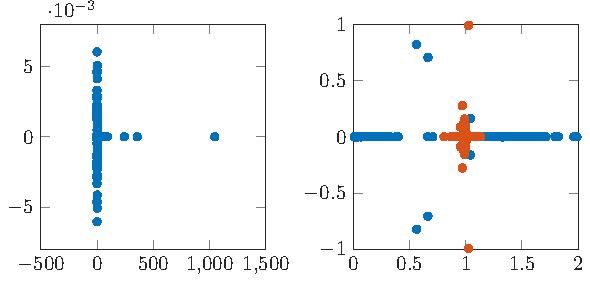
\includegraphics[scale=1]{../src/figure/spectraRajat12.pdf}
%% This file was created by matlab2tikz v0.4.7 running on MATLAB 8.5.
% Copyright (c) 2008--2014, Nico Schlömer <nico.schloemer@gmail.com>
% All rights reserved.
% Minimal pgfplots version: 1.3
% 
% The latest updates can be retrieved from
%   http://www.mathworks.com/matlabcentral/fileexchange/22022-matlab2tikz
% where you can also make suggestions and rate matlab2tikz.
% 
\documentclass[tikz]{standalone}
\usepackage{pgfplots}
\usepackage{grffile}
\pgfplotsset{compat=newest}
\usetikzlibrary{plotmarks}
\usepackage{amsmath}

\begin{document}
%
% defining custom colors
\definecolor{mycolor1}{rgb}{0.00000,0.44700,0.74100}%
\definecolor{mycolor2}{rgb}{0.85000,0.32500,0.09800}%
%
\begin{tikzpicture}

\begin{axis}[%
width=1.5in,
height=1.5in,
scale only axis,
separate axis lines,
every outer x axis line/.append style={white!15!black},
every x tick label/.append style={font=\color{white!15!black}},
xmin=-500,
xmax=1500,
every outer y axis line/.append style={white!15!black},
every y tick label/.append style={font=\color{white!15!black}},
ymin=-0.008,
ymax=0.008,
name=plot1
]
\addplot [color=mycolor1,only marks,mark=*,mark options={solid},forget plot]
  table[row sep=crcr]{1047.29815201591	0\\
357.877584204619	0\\
242.897308345831	0\\
92.2503566291336	0\\
78.6578597480995	0\\
50.472748737374	0\\
41.4322443693913	0\\
38.1713318245436	0\\
27.8950354612715	0\\
23.8259447172687	0\\
18.0045003280556	0\\
12.9945563119527	0\\
20.9038827402654	0\\
20.8978410930135	0\\
20.8976061965757	0\\
20.8961316850475	0\\
20.8958477048557	0\\
20.8953940404802	0\\
20.8955585715939	0\\
20.8955156760486	0\\
11.7522816126353	0\\
8.69389589518882	0\\
8.58425951078492	0\\
8.45466084906094	0\\
8.03343287264466	0\\
7.81359167200324	0\\
7.79943312064493	0\\
7.79104258326008	0\\
7.78451147724325	0\\
7.78081447163391	0\\
7.78146093598581	0\\
7.73057806320756	0\\
7.70508728558509	0\\
7.67271023029415	0\\
7.66864684933175	0\\
7.66188808348286	0\\
7.65836287939247	0\\
7.65426751514009	0\\
7.38838442630385	0\\
7.38939801011705	0\\
7.25443249875315	0\\
7.25658058047769	0\\
7.08590596725249	0\\
7.0665609266398	0\\
6.97885221080755	0\\
6.90350558270556	0\\
6.8430274042077	0\\
6.6483424406183	0\\
6.45155053279957	0\\
6.38383715723975	0\\
6.39551304848687	0\\
6.19690669290933	0\\
5.56241933481049	0\\
6.22518878202494	0\\
6.22509277817114	0\\
6.22509291183186	0\\
4.80572871494284	0\\
4.78489878193107	0\\
4.4837501026667	0\\
4.48429533513369	0\\
4.53471066091145	0\\
4.53471071483334	0\\
4.09176202923526	0\\
3.99030194464551	0\\
3.95428003986651	0\\
3.93197603285984	0\\
3.93100140205801	0\\
3.91363413089115	0\\
3.88671190509238	0\\
3.87724734578243	0\\
3.62240813759465	0.000592627946964726\\
3.62240813759465	-0.000592627946964726\\
3.62128569899305	0\\
3.73646405362475	0\\
3.7380622197238	0\\
3.73812275459653	0\\
3.73811702322689	0\\
3.73811703398977	0\\
3.28844118473144	0\\
3.3230259984888	0\\
3.31753634609856	0\\
3.30792225333134	0\\
3.30807015741629	0\\
3.33385796239175	0\\
3.33643121864808	0.000550198536066991\\
3.33643121864808	-0.000550198536066991\\
3.33644560473943	0.000551505576573188\\
3.33644560473943	-0.000551505576573188\\
3.18799618325145	0\\
3.17231794258786	0\\
3.17665039637194	0\\
3.17578919200791	0\\
3.11394358864351	0\\
2.97987322311844	0\\
2.83814038423009	0\\
2.83840204013647	0\\
2.76951356371019	0\\
2.74414064953716	0\\
2.70659628274085	0\\
2.70230384201893	0\\
2.69148253886648	0\\
2.69733655975391	0\\
2.69615387658857	0\\
2.62882339844446	0\\
-0.973197661254783	0\\
-0.96488326551753	0\\
-0.961423073460401	0\\
-0.940550098136274	0\\
-0.932188923334964	0\\
-0.930857249059903	0\\
2.38940056494511	0\\
2.3924245611743	0\\
2.42636212040177	0\\
2.62356911865025	0\\
2.62356911865024	0\\
2.62356911865022	0\\
2.41800097396139	0\\
2.41799944930682	0\\
2.41799919456066	9.48489589977536e-08\\
2.41799919456066	-9.48489589977536e-08\\
2.41799925957563	6.4790279539192e-08\\
2.41799925957563	-6.4790279539192e-08\\
2.53072958081398	0\\
2.51881649758084	0\\
2.48507778497835	0\\
2.4851816285265	0\\
2.48524380533502	0\\
2.51345690394745	0\\
2.51343186518185	0\\
2.51348213827995	0\\
2.57137112846056	0\\
2.55467386922797	0\\
2.58699114673978	0\\
2.58698820416011	0\\
2.58698820416009	0\\
2.56287331756127	0\\
2.57522228319018	1.33060955831366e-07\\
2.57522228319018	-1.33060955831366e-07\\
2.57522241457178	1.13577483991455e-07\\
2.57522241457178	-1.13577483991455e-07\\
2.57522290892544	0\\
2.57522303359597	0\\
2.5575323182388	0\\
2.56499307035301	0\\
2.56484509791272	0\\
2.56517144435785	0\\
2.56482401597514	0\\
2.56489323272368	0\\
2.48514830334495	0\\
2.48514830334496	0\\
2.48543632991154	0\\
2.48543632991154	0\\
2.48543632991156	0\\
2.50177830505643	0\\
2.55792295917424	0\\
2.55792409523134	0\\
2.55792407784614	3.64138982833187e-09\\
2.55792407784614	-3.64138982833187e-09\\
2.5579240808062	2.7987503921698e-09\\
2.5579240808062	-2.7987503921698e-09\\
2.55812079990539	0\\
2.55812206852104	0\\
2.55812206852105	0\\
2.55812206852104	0\\
2.50177830505645	0\\
2.50177830505642	1.72531658603426e-15\\
2.50177830505642	-1.72531658603426e-15\\
2.50177830505641	0\\
2.27925043404529	0\\
2.5869882041601	0\\
2.10332401220952	0\\
2.20723014756607	0\\
2.30180234646099	0\\
2.31265403638585	0\\
2.14703519301086	0\\
2.38945025880495	0\\
2.38934576727631	0\\
2.3925789209991	0\\
2.39224955564216	0\\
2.40023188134977	0\\
2.43990369149222	0\\
2.15938905622096	0\\
2.1582087649489	0\\
2.15836851438485	5.18359756313865e-05\\
2.15836851438485	-5.18359756313865e-05\\
2.15839972928559	2.97179636841567e-05\\
2.15839972928559	-2.97179636841567e-05\\
2.15840651560102	0\\
2.43989804365116	0\\
2.43989804365116	0\\
2.39868485326026	0\\
2.48514830334497	0\\
2.43989804365116	0\\
2.39868479583991	0\\
2.3094705467608	0\\
2.23982167008845	0\\
2.23982167008847	0\\
2.23982167008847	0\\
2.30946686886557	0\\
2.39868479583991	0\\
2.39868479583989	0\\
2.23581469665507	0\\
2.23581469665504	0\\
2.23581469665505	0\\
2.23581469665506	0\\
2.30936769494357	0\\
2.30936769494359	0\\
2.30936769494357	3.53183565073564e-15\\
2.30936769494357	-3.53183565073564e-15\\
2.30936769494358	0\\
2.30936769494358	7.50940934905391e-16\\
2.30936769494358	-7.50940934905391e-16\\
2.30936769494358	0\\
2.23982167008847	0\\
2.23581469665505	0\\
2.23581469665506	0\\
2.58698820416007	0\\
2.5869882041601	0\\
2.58698820416008	0\\
1.96838354303575	0\\
1.97402038187108	0\\
2.03396482025407	0\\
2.40023188134976	0\\
2.07676332416878	0\\
2.40023188134979	0\\
2.02147579149773	0\\
2.00490422758448	0\\
2.43989804365113	0\\
2.01004266518226	0\\
2.00986865994567	0\\
2.00963825738989	0\\
2.001899	0\\
2.00966774431608	0\\
2.07437821900955	0\\
2.07440930850519	0\\
2.01674460699738	0\\
2.07439379756181	1.99237810126539e-06\\
2.07439379756181	-1.99237810126539e-06\\
2.0743952091705	1.13869029913488e-06\\
2.0743952091705	-1.13869029913488e-06\\
2.01524916462385	0\\
2.01562045082657	8.20126127899655e-05\\
2.01562045082657	-8.20126127899655e-05\\
2.01566885927392	0\\
2.01559122095197	4.18595106137468e-05\\
2.01559122095197	-4.18595106137468e-05\\
2.07439385843246	0\\
2.01562044249151	0\\
2.48514830334496	0\\
2.48514830334494	0\\
2.48543632991151	0\\
2.48543632991155	0\\
2.48543632991153	0\\
2.39868479583991	0\\
2.00199100000002	0\\
2.001991	0\\
2.001991	0\\
2.00199099999999	0\\
2.55812206852102	0\\
2.55812206852107	0\\
1.83039090393522	0\\
1.80818248226548	0\\
2.01722799999999	0\\
1.75767129823596	0\\
1.79607613684557	0\\
1.79577317754079	0\\
1.79949162286513	0\\
1.77637709882398	0\\
1.78104583517032	0\\
1.78466525213699	0\\
1.79952695756303	0\\
1.79953222940716	0\\
1.78159246320547	0\\
1.78364390942789	0\\
1.78259405173869	0\\
1.78253134979333	0\\
2.43989804365116	0\\
2.50177830505644	1.69831466010162e-15\\
2.50177830505644	-1.69831466010162e-15\\
2.43989804365116	0\\
2.3986847958399	0\\
2.23982167008848	0\\
2.485148303345	0\\
2.23982167008847	0\\
2.23982167008847	0\\
2.48514830334497	0\\
2.30936769494357	0\\
2.55812206852105	0\\
2.3986847958399	0\\
1.71899997188283	0\\
2.50177830505641	0\\
2.50177830505644	0\\
1.73678388318871	0\\
1.70960941708888	0\\
1.69170287919692	0\\
1.71353081550794	0\\
1.71361454213427	0\\
-0.0540738017680939	0\\
1.70247382148826	0\\
1.64632794564593	0\\
1.71360196665082	6.09138869960357e-06\\
1.71360196665082	-6.09138869960357e-06\\
1.71360324036873	0\\
1.71359944693089	0\\
1.67715895198078	0\\
1.70245774119505	0\\
1.70251107900092	0\\
1.64781786172003	0\\
1.66769813113443	0\\
1.57159271271709	0\\
1.64484713481815	0\\
1.67471899662199	0\\
1.67473924357999	0\\
1.67473616140033	6.67775928094184e-07\\
1.67473616140033	-6.67775928094184e-07\\
1.67473535661913	3.70795199290703e-07\\
1.67473535661913	-3.70795199290703e-07\\
2.001991	0\\
1.68344330850776	0\\
2.001991	0\\
2.48543632991152	0\\
2.48543632991153	0\\
2.48543632991152	0\\
2.48514830334494	0\\
2.00199099999999	0\\
2.23581469665503	0\\
2.23581469665504	0\\
2.23581469665505	0\\
1.68344595634885	0\\
2.48514830334496	0\\
2.23982167008847	0\\
2.23982167008848	0\\
2.48543632991154	0\\
1.68344595634885	0\\
2.48514830334496	0\\
1.53699346082983	0\\
1.53462691106207	0\\
2.23581469665503	0\\
1.56188793147894	0\\
1.5618922000946	0\\
2.23982167008847	0\\
2.23982167008845	0\\
1.56188793147895	0\\
1.56188793147894	0\\
2.48514830334496	0\\
2.48543632991154	0\\
2.48543632991154	0\\
-0.0303729264020917	0\\
2.48514830334496	0\\
2.23581469665505	0\\
2.23982167008847	0\\
2.48543632991154	0\\
-0.0121691439268874	0\\
1.68344595634885	0\\
2.23581469665504	0\\
1.68344595634886	0\\
2.48514830334498	0\\
2.23581469665504	0\\
2.23982167008847	0\\
1.52282998402486	0\\
0.00151484438837924	0\\
0.00216377676307339	0\\
0.00216357913375383	0\\
0.00216312600570455	0\\
1.68344595634884	0\\
1.68344595634884	0\\
1.56188793147897	0\\
1.12327207382871	0\\
1.11799573508081	0\\
1.1163264181689	0\\
1.35290780504303	0\\
1.32060274541632	0\\
1.31480274974356	0\\
1.30945400158051	0\\
1.30709107729984	0.000510190738343425\\
1.30709107729984	-0.000510190738343425\\
1.37738835903844	0\\
1.30508540950403	0.00081919915192551\\
1.30508540950403	-0.00081919915192551\\
1.29885757056358	0\\
1.29004637608716	0.00506937807492582\\
1.29004637608716	-0.00506937807492582\\
1.29424207930395	0\\
1.27084986216149	0\\
1.29189832268228	0.00113788432126869\\
1.29189832268228	-0.00113788432126869\\
1.28316037573784	0.00413597293444821\\
1.28316037573784	-0.00413597293444821\\
1.28783756569988	0.000279737517306064\\
1.28783756569988	-0.000279737517306064\\
1.28429621406536	0.00112408090738493\\
1.28429621406536	-0.00112408090738493\\
1.27750371402873	0\\
1.28073034609523	0.00105191154975816\\
1.28073034609523	-0.00105191154975816\\
1.27937511036244	0.000877509529449312\\
1.27937511036244	-0.000877509529449312\\
1.17409215561352	0\\
1.36588835845446	0\\
1.27975471410879	0\\
1.17457131980386	0\\
1.36773607562829	0\\
1.17475959135781	0\\
1.36867072249787	4.41838135447583e-05\\
1.36867072249787	-4.41838135447583e-05\\
1.36829713662737	0.000119639521162384\\
1.36829713662737	-0.000119639521162384\\
1.2538599799777	0\\
1.25919940049345	0\\
1.36810992640469	0.00016828203797627\\
1.36810992640469	-0.00016828203797627\\
1.17497571287379	0\\
1.17442458206841	0\\
1.17442459550419	0\\
1.25322182253098	0\\
1.25875625080191	0\\
1.2587522804392	0\\
1.25874346711394	0\\
1.17442459733415	0\\
1.17497573842527	0\\
1.1749757381822	0\\
1.25873966794633	0\\
1.25874987470779	0\\
1.25873936101608	0\\
1.26424414922297	0\\
1.254141	0\\
1.29591911681129	0\\
1.56188793147894	0\\
1.46971574982736	0\\
1.45727949833402	0\\
1.09300996427239	0\\
1.08992465256625	0\\
1.08228212864556	0\\
1.07454171436372	0\\
0.101165247025547	0\\
0.0878262252211071	0\\
0.0853135257929892	0\\
0.0721147777647796	0.00225937121243828\\
0.0721147777647796	-0.00225937121243828\\
0.0714470286231587	0\\
0.00279967344210845	0\\
0.0660808408412388	0.00604197337708828\\
0.0660808408412388	-0.00604197337708828\\
0.0683317585510536	0\\
0.0662331892200689	0\\
0.0648416858950716	0\\
0.0619008065979152	0.00468073794363514\\
0.0619008065979152	-0.00468073794363514\\
0.00438641510961533	0\\
0.00324143119823489	0\\
0.00324027534128884	0\\
0.00324069675768951	0\\
0.0593322171253518	0.00331683288639802\\
0.0593322171253518	-0.00331683288639802\\
0.0616371555260422	0\\
0.0612106003827127	0\\
0.0564172102841073	0.00459481708538226\\
0.0564172102841073	-0.00459481708538226\\
0.00539916990551391	0\\
0.00540672190209602	0\\
0.0503427863905283	0.0020349460763053\\
0.0503427863905283	-0.0020349460763053\\
0.00613835537574439	0\\
0.0550389393445926	0\\
0.0543092218813553	0\\
0.0495069471563079	0\\
0.00620957168819345	0\\
0.00630157281124272	0\\
0.00627397133070505	0\\
0.0534428479942885	0\\
0.0530491270483553	0\\
0.00624735792021986	0\\
1.56188793147896	0\\
1.07472338505292	0\\
1.39662684533634	0\\
1.06464956321414	0\\
1.06425985487024	0\\
1.39581538077026	0\\
0.113112207208825	0\\
0.110226892756942	0\\
0.102469947140756	0\\
0.103599125912632	0\\
0.1069752679669	0\\
0.00815918178466247	0\\
0.105827366153688	0\\
0.105866209116103	0\\
0.0480722508430099	0\\
0.105855704120627	0\\
0.105861718728751	0\\
0.0473319171168267	0\\
0.0441180695613959	0\\
0.0461916938987973	0\\
0.0452368511208848	0\\
0.0433753639547137	0\\
0.0402783037721536	0\\
0.0414484977441486	0\\
0.0421741737283128	0\\
0.0428237207553945	0\\
0.00882144859094285	0\\
0.0118263325556242	0.00205400422645578\\
0.0118263325556242	-0.00205400422645578\\
0.0379210349381931	0\\
0.0367886225627002	0\\
0.0131083613950181	0.0022924104616651\\
0.0131083613950181	-0.0022924104616651\\
0.0121487861461946	0.00217766314292044\\
0.0121487861461946	-0.00217766314292044\\
0.00933612478646947	0\\
0.00937382025761187	0\\
0.00947642452834763	0\\
0.00961120592216643	0\\
0.0357425838997141	0\\
0.0352220537607784	0\\
0.034608761988822	0\\
0.0341114288157059	0\\
0.0337590510038848	0\\
0.0335425142610698	0\\
0.0340243439999901	0\\
0.0326736282436509	0\\
0.0332422770486953	0\\
0.0320966060867822	0\\
0.0312184106141097	0\\
0.0315612120327166	0\\
0.0131755745623868	0\\
0.0292288694429035	0\\
0.0285805229198341	0\\
0.0138894890012035	0.000173675586650346\\
0.0138894890012035	-0.000173675586650346\\
0.0136624047406229	0\\
0.0283931335004348	0\\
0.0148501543675317	0\\
0.0115390159788551	0\\
0.0125228884088101	0\\
0.0306438389097043	0\\
0.0125675278261072	0\\
0.0150592027277706	0\\
0.0113161432855532	0\\
0.0259754991706454	0\\
0.0266888005095972	0\\
0.0264518747966583	0\\
0.0271700810748023	0\\
0.0274318016337753	0\\
0.0261798369088573	0\\
0.0303315642520237	0\\
0.0105586198937823	0\\
0.0305189811645744	0\\
0.011160282459259	0\\
0.0307088265158133	0\\
0.0197703407007433	0\\
0.010980872147251	0\\
0.0301064471455244	0\\
0.023902610789077	0\\
0.0162107455500884	0\\
0.0186584657934122	0.000479793267178386\\
0.0186584657934122	-0.000479793267178386\\
0.0195625064874657	0\\
0.016419763470792	0\\
0.0232680050864907	0\\
0.0106600872013739	0\\
0.0210216014589702	0\\
0.0234317096925321	0\\
0.0235562540101919	0\\
0.0217107204971371	0\\
0.0212999798813712	0\\
0.017837378544155	0\\
0.0176328350866841	0\\
0.0183728500543098	0\\
0.0106925632809727	0\\
0.0212397307821441	0\\
0.0169257398526956	0\\
0.0225063423719254	0\\
0.0107431709747227	0\\
0.0173092697490551	0\\
0.0222020694432736	0\\
0.022218939641998	0\\
0.0107336947118359	0\\
0.010726849650936	0\\
0.0107639455215826	0\\
0.0222640950140864	0\\
0.0171081245473013	0\\
0.0171130990743177	0\\
0.0171153948760084	0\\
0.131774046825401	0\\
0.147356106939653	0\\
0.148943448242304	0.00144574473933474\\
0.148943448242304	-0.00144574473933474\\
0.1275941618398	0\\
0.126656225538086	0\\
0.126241942392529	0\\
0.12564335370635	0\\
0.127032129049197	0\\
0.175740303142317	0.00128187738549756\\
0.175740303142317	-0.00128187738549756\\
0.176062173289051	0.000204427787333508\\
0.176062173289051	-0.000204427787333508\\
0.153116901078569	0\\
0.175678853498852	0.00121148127079727\\
0.175678853498852	-0.00121148127079727\\
0.175678511746177	0.00121156197167992\\
0.175678511746177	-0.00121156197167992\\
0.160166008137793	0\\
0.160373958027923	0\\
0.125769749755925	0\\
0.125769616169133	0\\
0.125769603376137	0\\
0.141478598571609	0\\
0.16156524550349	0\\
0.161565628438919	0\\
0.16156558030344	0\\
0.161241439208609	0\\
0.148428098236388	0.0020988732348131\\
0.148428098236388	-0.0020988732348131\\
0.148427992661289	0.00209874416624439\\
0.148427992661289	-0.00209874416624439\\
0.125498615469723	0\\
0.148428085497381	0.00209878020338101\\
0.148428085497381	-0.00209878020338101\\
0.161239465321307	0\\
0.161239487862374	0\\
0.141648184579833	0\\
0.126962113227985	0\\
0.126962113151331	0\\
0.141648094290163	0\\
0.141648060791423	0\\
0.12549861518132	0\\
0.141536705163429	0\\
0.141536704034602	0\\
0.1415367036867	0\\
1.40146767480166	0\\
1.39806799999999	0\\
1.04034519870323	0\\
1.26424414922299	0\\
1.26424414922298	0\\
1.44628640104724	0\\
1.40437376619245	0\\
1.25322182253098	0\\
1.03654588592006	0\\
1.02934394475446	0\\
1.02748019252403	0\\
1.39515101195782	0\\
1.39573338217988	0\\
1.39806799999999	0\\
0.191329930503368	0\\
0.189487497173342	0\\
0.18898384573082	0\\
0.189747627845536	0\\
0.188946979278089	0\\
0.189749923187435	0\\
0.189089635553542	0\\
1.39747072738675	0\\
1.41314508000093	0\\
1.39955506892609	0\\
1.40109200000001	0\\
1.00716794168582	0\\
1.00068877332897	0.00142723157246915\\
1.00068877332897	-0.00142723157246915\\
1.00227456935376	0\\
0.997019749691468	0\\
0.999223328760453	0\\
1.005097	0\\
1.001288	0\\
0.993383300805879	0\\
0.992201466608634	0\\
0.992194744790113	0\\
0.992194298907179	0\\
0.992193402225829	0\\
0.992193389686704	0\\
0.202016279335528	0\\
0.200538613515774	0\\
0.211215455983605	0\\
0.992193136676476	0\\
0.201215960242455	0\\
0.210166205977828	0\\
0.210248232362813	0\\
0.210223965574603	0\\
0.189096762294451	0\\
0.189096214308457	0\\
0.18909626018169	0\\
1.39806800000001	0\\
0.933673052197648	0\\
0.933668309076653	0\\
0.933555229007951	0\\
0.933560847989067	0\\
0.895864206140914	0\\
0.90432200071696	0\\
0.950267839722649	0\\
0.904047371079272	0\\
0.903940199990178	0\\
0.903943834896707	0\\
0.999230998873767	0\\
0.999228994881999	0\\
0.999228994881992	0\\
0.979176248989525	0\\
0.978334395441459	0\\
0.981639498706639	0\\
0.238692094451114	0\\
0.212169634795656	0\\
0.215233980017176	0\\
0.214447215792916	0\\
0.214583455111043	0\\
0.214855925151826	0\\
0.974209794073522	0\\
0.217429088035297	0\\
0.975249789193535	0\\
0.992195005118004	0\\
0.992194999909509	0\\
0.221428150716044	0\\
0.212033219995734	0\\
0.212025046802496	0\\
0.212028627925555	0\\
0.220032316111768	0\\
0.224439042121476	0\\
0.219433632434835	0\\
0.224416649718101	0\\
0.976188616160567	0\\
0.219178151888548	0\\
0.224418274383455	0\\
0.976219556550999	0\\
0.219243014633053	0\\
0.21919417898976	0\\
0.219232064731579	0\\
0.224418058599617	0\\
0.976213545096567	0\\
0.97621355202219	0\\
0.976213554656252	0\\
0.97621355904438	0\\
0.976213557973255	0\\
0.976213530941144	0\\
0.801310297823268	0\\
0.819624967089265	0.00193201327126144\\
0.819624967089265	-0.00193201327126144\\
0.815291562043101	0\\
0.880402479679904	0\\
0.913540030685646	0\\
0.814937047476259	0\\
0.913540030756044	0\\
0.819749310936882	0\\
0.897903999999991	0\\
0.896123241864633	0\\
0.879158933475548	0\\
0.879174912200584	0\\
0.992194999909539	0\\
0.992195005118018	0\\
0.978357228202162	0\\
0.978362	0\\
0.201217	0\\
0.978361000000004	0\\
0.269986587354777	0\\
0.243349274186282	0\\
0.262020165076691	0\\
0.24120529595454	0\\
0.248460631079261	0\\
0.978361	0\\
0.256340432972094	0\\
0.255537370889298	0\\
0.237901113363325	0\\
0.252123827231797	0\\
0.252208556188299	0\\
0.252220835361518	0\\
0.240276375590333	0\\
0.253862010237017	0\\
0.240275496873895	0\\
0.253844503344792	0\\
0.97613939638956	0\\
0.976172285245957	0\\
0.253838052781512	0\\
0.216876819325269	0\\
0.216876808451397	0\\
0.220464201035977	0\\
0.220462884417992	0\\
0.220462686097114	0\\
0.756605781250219	0\\
0.760427212576682	0\\
0.761990864851067	0\\
0.761905893169722	0\\
0.796988101928661	0\\
0.798266197076626	0\\
0.804355898071338	0\\
0.875922840802158	0\\
0.893726858932193	0\\
0.893386988042188	0\\
0.870932535343551	0\\
0.816617920286521	0\\
0.968462307003575	0.00279174196203083\\
0.968462307003575	-0.00279174196203083\\
0.252130661791823	0\\
0.814937999061162	0\\
0.814927999999999	0\\
0.814906999999999	0\\
0.240275498677919	0\\
0.253836647542861	0\\
0.259745172794204	0\\
0.259745116354243	0\\
0.913542000000007	0\\
0.971148509355034	0\\
0.969061442175419	0\\
0.237901058203542	0\\
0.969292515232857	0\\
0.969665853265798	0\\
0.237901058476379	0\\
0.97618090186226	0\\
0.970027932920328	0\\
0.913537000024168	0\\
0.913537000024176	0\\
0.975831000000001	0\\
0.259745080015556	0\\
0.975831000000023	0\\
0.972133999999993	0\\
0.972133999999995	0\\
0.274280952337474	0\\
0.274261016559466	0\\
0.75457936192138	0\\
0.87074100364971	0\\
0.819717097125052	0\\
0.870715096566695	0\\
0.81661790287494	0\\
0.961204617820135	0\\
0.967581525207745	0\\
0.969846038015764	0\\
0.913541999999998	0\\
0.971175000000007	0\\
0.976172285245953	0\\
0.286395267754998	0\\
0.286834276112618	0\\
0.286600344716162	0\\
0.719564489181893	0\\
0.75328457412182	0\\
0.744037393201458	0\\
0.279517648147048	0\\
0.279517963641087	0\\
0.274260777875094	0\\
0.740636186282975	0.00293515590005815\\
0.740636186282975	-0.00293515590005815\\
0.279517938818714	0\\
0.274260768594419	0\\
0.747542242088367	0\\
0.842618476460064	0\\
0.819717097125061	0\\
0.842618476460063	0\\
0.968075821960332	0\\
0.968186584127521	0\\
0.970134311293349	0\\
0.971174771797849	0\\
0.971175000000002	0\\
0.331867062782502	0\\
0.30788035080711	0\\
0.31765110003756	0\\
0.306903786888953	0\\
0.314553435870879	0\\
0.269386168029699	0\\
0.323167756016441	0\\
0.316083633809835	0\\
0.859667603242479	0\\
0.716460972239661	0\\
0.71881980146396	0\\
0.706014959045501	0\\
0.73267558607203	0\\
0.713429205353227	0\\
0.71342455337034	0\\
0.746497068400267	0\\
0.746544410710052	0\\
0.816617902874956	0\\
0.737806178890187	0\\
0.746634122315675	0\\
0.962192000000004	0\\
0.737100899954064	0\\
0.737091268963304	0\\
0.978361000000023	0\\
0.737088054623992	0\\
0.972134000000011	0\\
0.975831000000011	0\\
0.29509489523134	0\\
0.344682448494195	0\\
0.34379245093636	0\\
0.340129852336095	0\\
0.322327793299608	0.000491201197012275\\
0.322327793299608	-0.000491201197012275\\
0.321953115356046	0\\
0.307037947767293	0\\
0.269386161727381	0\\
0.307037838585893	0\\
0.269386161728689	0\\
0.322064294330546	0\\
0.699147810389602	0\\
0.865586949420331	0.000473844474179893\\
0.865586949420331	-0.000473844474179893\\
0.865436996567366	0.00144590654803521\\
0.865436996567366	-0.00144590654803521\\
0.721696999999999	0\\
0.861336029467733	0\\
0.861724190487376	0\\
0.861549507427448	0\\
0.315741656818759	0\\
0.3157416566887	0\\
0.966345603610447	0\\
0.740888942637126	0\\
0.968275323923124	0\\
0.739965057362871	0\\
0.746226271689497	0\\
0.968423275158581	0\\
0.968422314477488	0\\
1.43080970999075	0\\
1.43090957119257	0\\
1.43092193107392	0\\
1.43090975813538	0\\
0.624836480515241	0\\
0.698337842104806	0\\
0.696355395462444	0\\
0.696006432478648	0\\
0.731310999999994	0\\
0.754454622926217	0\\
0.754454622926215	0\\
0.972134000000015	0\\
0.536972417172604	0\\
0.555924009273426	0\\
0.556058021515436	0\\
0.570452697872551	0\\
0.605264869654607	0\\
0.601297416534931	0\\
0.581111740609022	0\\
0.734986501159521	0\\
0.857350002130363	0\\
0.647244069222716	0\\
0.657301465323675	0\\
0.657771019230083	0\\
0.641259378822331	0\\
0.642781241365314	0\\
0.644427599772787	0\\
0.645191464027944	0\\
0.635460919439466	0\\
0.636167174338885	0\\
0.636239729694589	0\\
0.637364736107778	0\\
0.868506000000005	0\\
0.963943098137745	0\\
0.638504430790353	0\\
0.868506000000013	0\\
0.968428755294666	0\\
0.638251362638061	0\\
0.636337650867206	0\\
0.637988839542753	0\\
0.638007237430409	0\\
0.545705414697204	0\\
0.862869803180989	0\\
0.862716368127316	0\\
0.863049938527922	0\\
0.862944502397056	0\\
0.735371109343873	0\\
0.588010307323467	0\\
0.580998810285612	0\\
0.580026305418979	0\\
0.602796449707942	0\\
0.573369652937088	0\\
0.575572941787816	0\\
0.751402000000001	0\\
0.59237126023082	0\\
0.575125549626249	0\\
0.645398330671987	0\\
0.592257956514269	0\\
0.751402000000012	0\\
0.645401921211344	0\\
0.734993999999992	0\\
0.968426573797986	0\\
0.573873934020201	0\\
0.968427096652568	0\\
0.968426904257903	0\\
0.968426960722119	0\\
0.857350002500044	0\\
0.857350002500207	0\\
0.857350002500127	0\\
0.748567999999997	0\\
0.748568000000006	0\\
0.734986890656137	0\\
0.636336404527348	0\\
0.577408000000005	0\\
0.57706423415319	0\\
0.577078162509147	0\\
0.577086240968999	0\\
0.577092156012862	0\\
0.292422501991048	0\\
0.291949302585839	0\\
0.322117715534608	0\\
0.322117715534611	0\\
0.366597744503441	0\\
0.363157464911496	0\\
0.36280609190706	0\\
0.362250543279566	0\\
0.362277533297456	0\\
0.602796407809301	0\\
0.865220999999997	0\\
0.964406714754054	0\\
0.865221000000004	0\\
0.292948754319442	0\\
0.292120551093045	0\\
0.292107752504453	0\\
0.366465699974764	0\\
0.862591250172633	0\\
0.666152034435648	0\\
0.666167856027548	0\\
0.420811507453728	0\\
0.964406714754056	0\\
0.573874999999996	0\\
0.573208501293367	0\\
0.416376901778796	0\\
0.416305736465692	0\\
0.430261569187622	0\\
0.435164622636679	0\\
0.447427948214672	0\\
0.443986098782071	0\\
0.445211335383905	0\\
0.441378688524099	0\\
0.448737954047533	0\\
0.548669284465392	0\\
0.440329942870283	0\\
0.448835170496973	0\\
0.963302001136489	0\\
0.963302001297305	0\\
0.963302002613777	0\\
0.448978467038364	0\\
0.963302000248314	0\\
0.453664565342141	0\\
0.548669284465389	0\\
0.453666891269282	0\\
0.438329686818335	0\\
0.438337990790866	0\\
0.438251392959166	0\\
0.438244995921265	0\\
1.43081127261327	0\\
1.43080914106782	0\\
0.292938109502631	0\\
0.292945186200773	0\\
0.292946377152244	0\\
0.682280011566339	0.00271872610564849\\
0.682280011566339	-0.00271872610564849\\
0.51852817657321	0\\
0.515221400152291	0\\
0.516232515094491	0\\
0.40856207089385	0\\
0.453667656257618	0\\
0.971175000000014	0\\
0.669179339775687	0\\
0.292134155637534	0\\
0.682200102338298	0.00273028778404557\\
0.682200102338298	-0.00273028778404557\\
0.680560397178577	0\\
0.677155874026466	0\\
0.382543037427623	0\\
0.393393873790661	0\\
0.430545000000001	0\\
0.372163545753519	0\\
0.374699100407165	0\\
0.378983696749496	0\\
0.373602706358788	0\\
0.467217137746485	0\\
0.37346108518533	0\\
0.37893536364988	0\\
0.964406714754062	0\\
0.96440671475405	0\\
0.684854000000002	0\\
0.681540476879809	0\\
0.675302300492991	0\\
0.675209484814003	0\\
0.683332081808756	0\\
0.687540177469023	0\\
0.687540177469022	0\\
0.674094541166223	0\\
0.519191802923382	0\\
0.673899799067417	0\\
0.512425815776982	0\\
0.511932931194846	0\\
0.511765108658964	0\\
0.511229522196866	0\\
0.673899301704352	0\\
0.511346290921004	0\\
0.511278622909537	0\\
0.435525728310505	0\\
0.442890408459265	0\\
0.503699010425849	0\\
0.680018844182836	0\\
0.680018777102811	0\\
0.680018733970146	0\\
0.474589731740656	0.00180670102373077\\
0.474589731740656	-0.00180670102373077\\
0.472570890628895	0\\
0.473328058786867	0\\
0.395375854042261	0\\
0.402319093220356	0\\
0.504441053313687	0\\
0.504438828765396	0\\
0.504451130674149	0\\
0.504450400910703	0\\
0.400113839156086	0\\
0.403960842375144	0\\
0.372806202411701	0\\
0.403960869636547	0\\
0.377283726762154	0\\
0.372870411617789	0\\
0.377785479582503	0\\
0.37776985926618	0\\
0.377162836434946	0\\
0.372872225063631	0\\
0.372870649041823	0\\
0.394385086369097	0\\
0.394385081482033	0\\
0.394385088385079	0\\
0.396027727778573	0\\
0.377168519169216	0\\
0.396027725379071	0\\
0.396027725343455	0\\
0.377528713887419	0\\
0.377552386160108	0\\
0.377454108608549	0\\
0.377453488470115	0\\
0.976172285245958	0\\
0.594377786661794	0\\
0.594384362416542	0\\
0.687381946235312	0\\
0.673900120630687	0\\
0.474748045962256	0.00172959105955868\\
0.474748045962256	-0.00172959105955868\\
0.403960875341788	0\\
0.687381946235311	0\\
0.292941000000006	0\\
0.292939999975832	0\\
0.292939999975833	0\\
0.475928310509443	0.0015235068869472\\
0.475928310509443	-0.0015235068869472\\
0.292941000000004	0\\
0.475356267804666	0.00152686560547191\\
0.475356267804666	-0.00152686560547191\\
0.594343001126237	0\\
0.401790327082603	0\\
0.292134858203728	0\\
0.29213485820373	0\\
0.594399918607112	0\\
0.473350223899687	0\\
0.594397737988191	0\\
0.474406931703463	0\\
0.292134858203731	0\\
0.594398950478643	0\\
0.594393168337928	0\\
0.594395579447904	0\\
0.679843000000002	0\\
0.674909918191252	0\\
0.67426957775239	0\\
0.674269541046652	0\\
0.494330434409287	0\\
0.513626622256695	0\\
0.513652524942665	0\\
0.401882016080218	0\\
0.674269530168663	0\\
0.669539001534683	0\\
0.401881479439902	0\\
0.513661234360807	0\\
0.478145259954437	0\\
0.513637693463795	0\\
0.474169017470985	0\\
0.669539002492166	0\\
0.669539002492179	0\\
0.474206588373963	0\\
0.372744506952533	0\\
0.372744507271119	0\\
0.372744507381837	0\\
0.594395003999536	0\\
0.377582848358882	0\\
0.377583155250046	0\\
0.377583114883676	0\\
0.370611	0\\
0.494229343962284	0\\
0.975831000000015	0\\
0.975831000000004	0\\
0.863416071797837	0\\
0.863400122206632	0\\
0.863434419456501	0\\
0.491668984308719	0\\
0.491763342915696	0\\
0.44287937707379	0\\
0.442879377073794	0\\
0.682418195106182	0\\
0.682418195106159	0\\
0.370611000000003	0\\
0.681551804893852	0\\
0.68155180489382	0\\
0.677349000000004	0\\
0.677349	0\\
0.370611000000003	0\\
0.370610999999997	0\\
0.971175000000012	0\\
0.29213485820373	0\\
0.292941000000001	0\\
0.59439099998913	0\\
0.51359400063237	0\\
0.669539002492193	0\\
0.488974143469006	0\\
0.513594000943271	0\\
0.490705087464749	0\\
0.491083996767176	0\\
0.491240060646091	0\\
0.491233805046448	0\\
0.483096418591015	0\\
0.482946510008681	0\\
0.482639869926366	0\\
0.482631839026095	0\\
0.483545952202159	0\\
0.483812109310645	0\\
0.863407590326353	0\\
0.400999808787206	0\\
0.4010601910409	0\\
0.863436003771566	0\\
0.863407590326356	0\\
0.863439520352204	0\\
0.401004790279985	0\\
0.401034899043261	0\\
0.401016060666819	0\\
0.401013944399058	0\\
0.401035831225845	0\\
0.863439044343176	0\\
0.863432409673638	0\\
0.863441999056734	0\\
0.863441999056739	0\\
0.863432409673649	0\\
0.401020459208338	0\\
0.863439998633238	0\\
0.863439998639017	0\\
0.401171044531799	0\\
0.401171044796953	0\\
0.863439999972161	0\\
0.863439997451994	0\\
0.863439998637915	0\\
0.401171044449271	0\\
0.594390999990135	0\\
0.485889009314871	0\\
0.673598000000001	0\\
0.673598000000005	0\\
0.673598000000005	0\\
0.5943910000905	0\\
0.594391000090496	0\\
0.513594000943266	0\\
0.401116053764693	0\\
0.401116053764691	0\\
0.494603523539938	0\\
0.494603523539939	0\\
0.50101214179627	0\\
0.501012141796276	0\\
0.50101214179628	0\\
0.48391711820843	0\\
0.401045850777021	0\\
0.401045850777024	0\\
0.484759509273241	0\\
0.48481897585319	0\\
0.484858044935996	0\\
0.48485075412981	0\\
0.48484576670468	0\\
0.490815999999999	0\\
0.490816000000003	0\\
0.484789645004308	0\\
0.484788683302951	0\\
0.481202000000002	0\\
0.481202	0\\
0.481201999999999	0\\
0.483913999999998	0\\
0.484745000938849	0\\
0.483914000000002	0\\
0.501012141796269	0\\
0.490816000000003	0\\
0.978361000000004	0\\
0.976172285245949	0\\
0.963302005122959	0\\
0.963302005122957	0\\
0.963302005122953	0\\
0.96330200512296	0\\
0.970133994877047	0\\
0.970133994877041	0\\
0.97013399487705	0\\
0.970133994877048	0\\
0.970133994877047	0\\
0.970133994877045	0\\
0.970133994877043	0\\
0.401045850777023	0\\
0.978360999999998	0\\
0.978361	0\\
0.964406714754043	0\\
0.972133999999995	0\\
0.971175000000001	0\\
0.971175000000005	0\\
0.964406714754052	0\\
0.964406714754045	0\\
0.976172285245954	0\\
0.976172285245952	0\\
0.971175000000003	0\\
0.976172285245953	0\\
0.490816	0\\
0.963302005122955	0\\
0.963302005122948	0\\
0.483914000000001	0\\
0.490816	0\\
0.970133994877051	0\\
0.970133994877052	0\\
0.970133994877055	0\\
0.963302005122957	0\\
0.963302005122954	0\\
0.963302005122954	0\\
0.487542916766038	0\\
0.487542916766031	6.17662903761969e-15\\
0.487542916766031	-6.17662903761969e-15\\
0.48754291676602	5.75250626287894e-15\\
0.48754291676602	-5.75250626287894e-15\\
0.487542916766013	0\\
0.487542916766015	0\\
0.48754291676603	0\\
0.487542916766023	1.00266416659325e-15\\
0.487542916766023	-1.00266416659325e-15\\
0.486774083233991	0\\
0.486774083233964	0\\
0.486774083233982	5.90613605945051e-15\\
0.486774083233982	-5.90613605945051e-15\\
0.486774083233987	0\\
0.486774083233973	4.28425988263879e-15\\
0.486774083233973	-4.28425988263879e-15\\
0.486774083233974	0\\
0.48677408323398	2.02596690433928e-15\\
0.48677408323398	-2.02596690433928e-15\\
0.486774083233978	0\\
0.963302005122961	0\\
0.963302005122965	0\\
0.486774083233987	0\\
0.96330200512295	0\\
0.487542916766024	0\\
0.963302005122955	0\\
1.42984800000006	0\\
1.42984799999994	0\\
1.42984799999995	0\\
1.42984800000006	0\\
1.42984800000006	0\\
1.42984799999995	0\\
1.42984799999995	0\\
1.42984800000005	0\\
1.42984800000006	0\\
1.42984800000005	0\\
1.42984799999995	0\\
1.42984799999995	0\\
1.42984799999995	0\\
1.42984799999995	0\\
1.42984799999996	0\\
1.42984800000004	0\\
1.42984800000005	0\\
1.42984800000005	0\\
1.42984800000004	0\\
1.42984800000005	0\\
1.42984800000004	0\\
1.42984799999996	0\\
1.42984799999996	0\\
1.42984799999996	0\\
1.42984799999996	0\\
1.42984799999997	0\\
1.42984800000005	0\\
1.42984800000004	0\\
1.42984800000004	0\\
1.42984800000004	0\\
1.42984800000004	0\\
1.42984799999996	0\\
1.42984799999997	0\\
1.42984799999997	0\\
1.42984800000004	0\\
1.42984800000004	0\\
1.42984799999998	0\\
1.42984799999997	0\\
1.42984800000002	0\\
1.42984800000003	0\\
1.42984800000003	0\\
1.42984800000003	0\\
1.42984799999997	0\\
1.42984799999998	0\\
1.42984799999998	0\\
1.42984800000004	0\\
1.42984800000003	0\\
1.42984800000003	0\\
1.42984800000001	0\\
1.42984800000002	0\\
1.42984799999998	0\\
1.42984799999998	0\\
1.42984800000002	0\\
1.42984800000002	0\\
1.42984799999998	0\\
1.42984799999999	0\\
1.42984800000003	0\\
1.42984800000001	0\\
1.42984800000002	0\\
1.42984800000002	0\\
1.42984799999998	0\\
1.42984800000003	0\\
1.42984800000001	0\\
1.42984800000001	0\\
1.429848	0\\
1.429848	0\\
1.42984799999999	0\\
1.42984799999999	0\\
1.42984800000002	0\\
1.42984799999998	0\\
1.429848	0\\
1.429848	0\\
1.42984799999999	0\\
1.42984799999999	0\\
1.42984799999999	0\\
1.42984800000001	0\\
1.429848	0\\
1.42984799999999	0\\
1.429848	0\\
1.42984800000001	0\\
1.42984799999999	0\\
1.429848	0\\
0.970133994877046	0\\
0.970133994877044	0\\
1.42984799999995	0\\
1.42984800000005	0\\
1.42984799999997	0\\
1.42984800000003	0\\
1.42984800000002	0\\
1.42984800000003	0\\
1.429848	0\\
1.42984800000003	0\\
0.963302005122957	0\\
0.970133994877045	0\\
0.97013399487705	0\\
1.42984799999996	0\\
1.42984799999997	0\\
1.42984799999996	0\\
1.42984799999998	0\\
1.42984800000003	0\\
1.42984800000002	0\\
1.42984799999997	0\\
1.42984800000002	0\\
1.42984799999998	0\\
1.42984799999999	0\\
1.42984800000001	0\\
1.429848	0\\
1.42984800000001	0\\
1.42984799999999	0\\
1.42984799999995	0\\
1.42984800000005	0\\
1.42984799999995	0\\
1.42984799999996	0\\
1.42984800000004	0\\
1.42984800000004	0\\
1.42984799999997	0\\
1.42984799999997	0\\
1.42984800000002	0\\
1.42984799999998	0\\
1.42984799999999	0\\
1.429848	0\\
1.429848	0\\
1.42984800000001	0\\
1.42984799999999	0\\
1.42984799999998	0\\
1.42984800000001	0\\
0.487542916766021	0\\
1.42984799999998	0\\
1.42984800000002	0\\
1.42984800000001	0\\
1.42984799999999	0\\
1.42984799999999	0\\
1.42984800000001	0\\
1.42984800000001	0\\
1.42984800000001	0\\
1.429848	0\\
1.42984799999996	0\\
1.42984800000004	0\\
1.42984799999996	0\\
1.42984800000004	0\\
1.42984800000004	0\\
1.42984800000004	0\\
1.42984800000003	0\\
1.42984800000003	0\\
1.42984800000003	0\\
1.42984800000001	0\\
1.42984799999998	0\\
1.42984799999999	0\\
1.42984799999999	0\\
1.42984800000002	0\\
1.429848	0\\
1.429848	0\\
1.429848	0\\
1.42984800000004	0\\
1.42984799999996	0\\
1.42984799999996	0\\
1.42984800000004	0\\
1.42984799999997	0\\
1.42984799999997	0\\
1.42984800000003	0\\
1.42984799999997	0\\
1.42984799999998	0\\
1.42984800000002	0\\
1.42984799999998	0\\
1.42984800000003	0\\
1.42984799999999	0\\
1.42984800000003	0\\
1.42984800000002	0\\
1.42984800000002	0\\
1.429848	0\\
1.42984799999999	0\\
1.42984800000001	0\\
1.42984800000001	0\\
1.42984800000001	0\\
1.42984800000001	0\\
1.42984800000002	0\\
1.42984800000001	0\\
1.42984800000001	0\\
1.429848	0\\
1.42984799999996	0\\
1.42984800000004	0\\
1.42984799999997	0\\
1.42984800000004	0\\
1.42984799999998	0\\
1.42984800000003	0\\
1.42984800000003	0\\
1.42984800000003	0\\
1.42984799999999	0\\
1.42984799999998	0\\
1.42984799999998	0\\
1.42984799999999	0\\
1.42984800000002	0\\
1.429848	0\\
1.429848	0\\
1.42984800000002	0\\
1.42984799999999	0\\
1.429848	0\\
1.42984800000001	0\\
1.42984800000004	0\\
1.42984799999998	0\\
1.42984800000003	0\\
1.42984799999998	0\\
1.42984799999999	0\\
1.42984799999999	0\\
1.42984799999999	0\\
1.42984800000001	0\\
1.42984799999999	0\\
1.429848	0\\
1.42984799999999	0\\
1.429848	0\\
1.429848	0\\
1.42984800000001	0\\
1.429848	0\\
1.429848	0\\
1.42984800000004	0\\
1.42984799999997	0\\
1.42984800000003	0\\
1.42984799999998	0\\
1.42984800000002	0\\
1.42984800000003	0\\
1.42984799999998	0\\
1.42984800000002	0\\
1.42984799999998	0\\
1.42984800000002	0\\
1.42984799999998	0\\
1.42984799999999	0\\
1.42984800000001	0\\
1.42984799999999	0\\
1.42984800000001	0\\
1.42984800000001	0\\
1.42984800000001	0\\
1.42984799999999	0\\
1.429848	0\\
1.42984799999999	0\\
1.42984800000001	0\\
1.429848	0\\
1.429848	0\\
1.429848	0\\
1.429848	0\\
1.42984799999998	0\\
1.42984800000003	0\\
1.42984800000003	0\\
1.42984800000003	0\\
1.42984800000003	0\\
1.42984800000002	0\\
1.42984800000002	0\\
1.42984799999999	0\\
1.42984799999999	0\\
1.42984800000002	0\\
1.42984799999999	0\\
1.42984800000002	0\\
1.42984799999999	0\\
1.42984800000001	0\\
1.42984800000002	0\\
1.42984800000001	0\\
1.42984799999999	0\\
1.42984800000001	0\\
1.429848	0\\
1.42984800000001	0\\
1.429848	0\\
1.429848	0\\
1.429848	0\\
1.429848	0\\
1.42984799999999	0\\
1.429848	0\\
1.429848	0\\
1.429848	0\\
1.429848	0\\
1.429848	0\\
1.429848	0\\
1.429848	0\\
1.429848	0\\
1.42984800000003	0\\
1.42984799999999	0\\
1.42984799999999	0\\
1.42984799999999	0\\
1.42984799999999	0\\
1.42984800000001	0\\
1.42984799999999	0\\
1.42984800000001	0\\
1.429848	0\\
1.42984799999999	0\\
1.42984800000001	0\\
1.429848	0\\
1.42984800000001	0\\
1.429848	0\\
1.429848	0\\
1.42984800000001	0\\
1.42984800000001	0\\
1.42984800000001	0\\
1.429848	0\\
1.42984800000001	0\\
1.429848	0\\
1.42984799999999	0\\
1.42984800000001	0\\
1.42984799999999	0\\
1.42984800000001	0\\
1.42984800000001	0\\
1.429848	0\\
1.42984800000001	0\\
1.429848	0\\
1.429848	0\\
1.429848	0\\
1.429848	0\\
1.42984800000001	0\\
1.42984800000001	0\\
1.429848	0\\
1.42984800000001	0\\
1.429848	0\\
1.429848	0\\
1.429848	0\\
1.429848	0\\
1.429848	0\\
1.429848	0\\
1.429848	0\\
1.42984800000001	0\\
1.42984799999999	0\\
1.429848	0\\
1.429848	0\\
1.42984799999999	0\\
1.429848	0\\
1.429848	0\\
1.42984799999999	0\\
1.42984799999999	0\\
1.42984799999999	0\\
1.42984800000001	0\\
1.42984799999999	0\\
1.42984800000001	0\\
1.42984799999999	0\\
1.429848	0\\
1.429848	0\\
1.42984800000001	0\\
1.42984800000001	0\\
1.42984799999999	0\\
1.42984799999999	0\\
1.429848	0\\
1.42984800000001	0\\
1.429848	0\\
1.429848	0\\
1.42984800000001	0\\
1.429848	0\\
1.429848	0\\
1.429848	0\\
1.42984799999999	0\\
1.429848	0\\
1.429848	0\\
1.42984799999999	0\\
1.429848	0\\
1.42984800000001	0\\
1.429848	0\\
1.429848	0\\
1.429848	0\\
1.429848	0\\
1.429848	0\\
1.429848	0\\
1.429848	0\\
1.42984800000001	0\\
1.429848	0\\
1.42984800000001	0\\
1.42984800000001	0\\
1.429848	0\\
1.429848	0\\
1.429848	0\\
1.429848	0\\
1.429848	0\\
1.429848	0\\
1.429848	0\\
1.42984799999999	0\\
1.429848	0\\
1.42984800000001	0\\
1.429848	0\\
1.42984800000001	0\\
1.429848	0\\
1.429848	0\\
1.429848	0\\
1.42984799999999	0\\
1.429848	0\\
1.429848	0\\
1.429848	0\\
1.429848	0\\
1.429848	0\\
1.429848	0\\
1.429848	0\\
1.429848	0\\
1.42984800000001	0\\
1.429848	0\\
1.42984800000001	0\\
1.42984799999999	0\\
1.429848	0\\
1.42984800000001	0\\
1.42984800000001	0\\
1.42984799999999	0\\
1.429848	0\\
1.429848	0\\
1.429848	0\\
1.429848	0\\
1.42984800000001	0\\
1.429848	0\\
1.429848	0\\
1.42984799999999	0\\
1.42984800000001	0\\
1.429848	0\\
1.429848	0\\
1.429848	0\\
1.429848	0\\
1.429848	0\\
1.429848	0\\
1.429848	0\\
1.429848	0\\
1.42984799999999	0\\
1.429848	0\\
1.429848	0\\
1.429848	0\\
1.429848	0\\
1.429848	0\\
1.429848	0\\
1.42984799999999	0\\
1.429848	0\\
1.42984799999999	0\\
1.42984800000001	0\\
1.429848	0\\
1.429848	0\\
1.42984799999999	0\\
1.42984799999999	0\\
1.429848	0\\
1.429848	0\\
1.429848	0\\
1.429848	0\\
1.429848	0\\
1.42984799999999	0\\
1.429848	0\\
1.429848	0\\
1.429848	0\\
1.429848	0\\
1.429848	0\\
1.429848	0\\
1.429848	0\\
1.429848	0\\
1.429848	0\\
1.429848	0\\
1.42984800000001	0\\
1.42984800000001	0\\
1.429848	0\\
1.429848	0\\
1.42984800000001	0\\
1.429848	0\\
1.429848	0\\
1.429848	0\\
1.429848	0\\
1.429848	0\\
1.429848	0\\
1.42984800000001	0\\
1.429848	0\\
1.429848	0\\
1.429848	0\\
1.429848	0\\
1.429848	0\\
1.429848	0\\
1.429848	0\\
1.429848	0\\
1.429848	0\\
1.429848	0\\
1.429848	0\\
1.429848	0\\
1.429848	0\\
1.429848	0\\
1.429848	0\\
1.429848	0\\
1.429848	0\\
1.429848	0\\
1.429848	0\\
1.429848	0\\
1.429848	0\\
1.429848	0\\
1.429848	0\\
1.429848	0\\
1.429848	0\\
1.429848	0\\
1.429848	0\\
1.429848	0\\
1.429848	0\\
1.429848	0\\
1.429848	0\\
1.429848	0\\
1.429848	0\\
1.429848	0\\
1.429848	0\\
1.429848	0\\
1.429848	0\\
1.429848	0\\
1.429848	0\\
1.429848	0\\
1.429848	0\\
1.429848	0\\
1.429848	0\\
1.429848	0\\
1.429848	0\\
1.429848	0\\
1.429848	0\\
1.429848	0\\
1.429848	0\\
1.429848	0\\
1.429848	0\\
1.429848	0\\
1.429848	0\\
1.429848	0\\
1.429848	0\\
1.429848	0\\
1.429848	0\\
1.429848	0\\
1.429848	0\\
1.429848	0\\
1.429848	0\\
1.429848	0\\
1.429848	0\\
1.429848	0\\
1.429848	0\\
1.429848	0\\
1.429848	0\\
1.429848	0\\
1.429848	0\\
1.429848	0\\
1.429848	0\\
1.429848	0\\
1.429848	0\\
1.429848	0\\
1.429848	0\\
1.429848	0\\
1.429848	0\\
1.429848	0\\
1.429848	0\\
1.429848	0\\
1.429848	0\\
1.429848	0\\
1.429848	0\\
1.429848	0\\
1.429848	0\\
1.429848	0\\
1.429848	0\\
1.429848	0\\
1.429848	0\\
1.429848	0\\
1.429848	0\\
1.429848	0\\
1.429848	0\\
1.429848	0\\
1.429848	0\\
1.429848	0\\
1.429848	0\\
1.429848	0\\
};
\end{axis}

\begin{axis}[%
width=1.5in,
height=1.5in,
scale only axis,
separate axis lines,
every outer x axis line/.append style={white!15!black},
every x tick label/.append style={font=\color{white!15!black}},
xmin=0,
xmax=2,
every outer y axis line/.append style={white!15!black},
every y tick label/.append style={font=\color{white!15!black}},
ymin=-1,
ymax=1,
at=(plot1.right of south east),
anchor=left of south west
]
\addplot [color=mycolor1,only marks,mark=*,mark options={solid},forget plot]
  table[row sep=crcr]{1	0\\
1	0\\
1	0\\
1	0\\
1	0\\
1	0\\
1	0\\
1	0\\
1	0\\
1	0\\
1	0\\
1	0\\
1	0\\
1	0\\
1	0\\
1	0\\
1	0\\
1	0\\
1	0\\
1	0\\
1	0\\
1	0\\
0.564008431415337	0.821062379289765\\
0.564008431415337	-0.821062379289765\\
1.96087482608671	0\\
1.98845980793013	0\\
1.98522954946746	0\\
1.97863620149343	0\\
1.98354170062951	0\\
1.98354145989318	0\\
1.9835415252496	0\\
1.9774092396717	0\\
1.97742424424528	0\\
1.97742194648719	0\\
1.97743697515721	0\\
1.97540591642362	0\\
1.97540598685027	0\\
1.97540599657838	0\\
0.663599322240126	0.705400568723788\\
0.663599322240126	-0.705400568723788\\
1.82324391174557	0\\
1.82148227900599	0\\
1.81102990027497	0\\
1.79662511345589	0\\
1.80241386039594	0\\
1.80204244225321	0\\
1.7984632418555	0\\
1.7995211531409	0\\
1.79292586523174	0\\
1.71034865703869	0\\
1.71119223570058	0\\
1.71151701524447	0\\
1.71152413230162	0\\
1.69532180857507	0\\
1.68817753406457	0\\
1.6857342461577	0\\
1.68150374077645	0\\
1.67901266591777	0\\
1.67666319235121	0\\
0.326682155505616	0\\
0.324700915711311	0\\
0.321716228983244	0\\
0.306727258341093	0\\
0.310391635396205	0\\
0.315358686017432	0\\
0.316240220561987	0\\
0.256582699102622	0\\
0.255159999429236	0\\
0.230928788191185	0\\
0.284707665618087	0\\
0.209216548116321	0\\
0.211116028480692	0\\
0.28701921048644	0\\
0.28638053398026	0\\
0.286173132800512	0\\
0.286045487066246	0\\
0.197046587996819	0\\
0.202647054240396	0\\
0.205860817043494	0\\
0.180822151208493	0\\
0.182879392880237	0\\
0.204426172133348	0\\
0.204576706852483	0\\
0.163661320671395	0\\
0.153095045375379	0\\
0.138152712747226	0\\
0.139847553374417	0\\
0.133010116043766	0\\
0.136466426263422	0\\
0.148746193890348	0\\
0.1486856874374	0\\
0.124128604784382	0\\
0.148703081638425	0\\
0.117823476528866	0\\
0.114421480415295	0\\
0.11679425846933	0\\
0.00983825057033696	0\\
0.00984901644182039	0\\
0.110542807969381	0\\
0.0114888949603424	0\\
0.0143033908842123	0\\
0.0143446637100639	0\\
0.0146455167773946	0\\
0.0149110682462934	0\\
0.0282083118584853	0.00457340334375753\\
0.0282083118584853	-0.00457340334375753\\
0.0294125468217194	0.00509297764270419\\
0.0294125468217194	-0.00509297764270419\\
0.019924350236525	0\\
0.019857701336762	0\\
0.0163269340856414	0\\
0.0298789822192574	0.00508382765080447\\
0.0298789822192574	-0.00508382765080447\\
0.0315582526743613	0\\
0.0254146120903828	0\\
0.0209982369345756	0\\
0.0163303179015716	0\\
0.0216639281782669	0\\
0.0163318036309112	0\\
0.0292340088985757	0\\
0.0219827981528402	0\\
0.0221280216772428	0\\
0.0268093759320719	0\\
0.0226413326422484	0\\
1.66672662254589	0\\
1.66663292540504	0\\
1.65923993106139	0\\
1.65735737826133	0\\
0.111519207679722	0\\
0.108242329636262	0\\
0.104385376626707	0\\
0.104077258453718	0\\
0.0920103731449088	0\\
0.0985665001588985	0\\
0.100053986534556	0\\
0.0908080422275462	0\\
0.0991820376206693	0\\
0.0997142453404691	0\\
0.0356209793175129	0\\
0.0372068122597716	0.00129529718011475\\
0.0372068122597716	-0.00129529718011475\\
0.0311018395966802	0\\
0.0386326490411593	0.00044230674635477\\
0.0386326490411593	-0.00044230674635477\\
0.0344524494433218	0\\
0.0347469482393616	0\\
0.0242144532462912	0\\
0.0242177331027651	0\\
0.0242261010811027	0\\
0.0903318605594133	0\\
0.0890046078749802	0\\
0.0866080235416246	0\\
0.0859024868502442	0\\
0.0835818451832572	0\\
0.0828461340564621	0\\
0.0813698214696139	0\\
0.0716187449320349	0.000648448125163102\\
0.0716187449320349	-0.000648448125163102\\
0.0778204826765886	0\\
0.0805232235908638	0\\
0.0798242511507389	0\\
0.0606012502875005	0\\
0.0754065246522833	0\\
0.0749994035010633	0\\
0.0747056672182721	0\\
0.0503250856595527	0\\
0.0486969383252463	0\\
0.0475802333739916	0\\
0.0492577419871124	0\\
0.044212952765984	0\\
0.0370136363887089	0\\
0.0426729882964387	0\\
0.0422721688872905	0\\
0.0418380641683301	0\\
0.0402961958312755	0\\
0.041165109515694	0\\
0.0406485324116298	0\\
0.0408289709286973	0\\
0.0409454906123569	0\\
0.0821049941891113	0\\
0.0791576049786058	0\\
0.0809159498424646	0\\
0.07056000112616	0\\
0.0517724564344929	0\\
0.0626775916781507	0\\
0.0684660252936447	0\\
0.0528976787069611	0\\
0.0528375379006873	0\\
0.0688227582173961	0\\
0.0645862755752918	0\\
0.0676185409108714	0\\
0.0680811187126194	0\\
0.0535247075227336	0\\
0.0580077476447008	0\\
0.0593245634843905	0\\
0.0587089378498832	0\\
0.0670068579016591	0\\
0.0560585000551342	0\\
0.0576255371326587	0\\
0.0653623372097751	0\\
0.0566895858903398	0\\
0.0543345452995777	0\\
0.0659612865008609	0\\
0.0575991510956891	0\\
0.0661437847579973	0\\
0.0655378935218396	0\\
0.0568935068363642	0\\
0.0550015300392235	0\\
0.0543331733175726	0\\
0.0665893786354927	0\\
0.0663216142809439	0\\
1.63546397969937	0\\
1.56793781727308	0\\
1.60865123079617	0\\
1.60880611279411	0\\
1.53603404784854	0\\
0.39863619968485	0\\
0.380496701286615	0\\
1.56344779810749	0\\
1.56049472288119	0\\
1.53384002907133	0\\
1.53694198112582	0\\
1.49804734491144	0\\
0.661169077848112	0\\
0.661246603416495	0\\
0.661221837794554	0\\
0.661208979499667	0\\
1.48695840920378	0\\
1.48692960663859	0\\
1.48693341601181	0\\
0.705969260305089	0\\
1.46826685363255	0\\
1.46488802907231	0\\
1.46082384288372	0\\
1.45807147267297	0\\
1.46365286131758	0\\
1.46394708541041	0\\
1.45660070806029	0\\
1.46385565608865	0\\
1.4643367563257	0\\
1.46433661542741	0\\
1.45128946722452	0\\
1.45508779846322	0\\
1.45743106285062	0\\
1.45743469618886	0\\
1.44536750261973	0\\
1.43800891121907	0\\
1.43759700986478	0\\
1.43514881374315	0\\
1.43499221443748	0\\
1.42967604386254	0\\
1.42861351104553	0\\
1.42893466390784	0\\
1.40964448822806	0\\
1.42017217176081	0\\
1.42612256959081	0\\
1.43204456857796	0\\
1.42929526576154	0\\
1.41557679464043	0\\
1.40349390819028	0\\
1.42570912586034	0\\
1.42657918618804	0\\
1.41179377337444	0\\
1.41532157352707	0\\
1.41529488119868	0\\
1.41520820920332	0\\
1.41521228742593	0\\
1.43961654537197	0\\
1.4292266265102	0\\
1.38609419409081	0\\
1.37535277623907	0\\
1.3825311260334	0\\
1.37340104154165	0\\
1.37439789659718	0\\
1.36786182500738	0\\
1.04066356403741	0.160788130378157\\
1.04066356403741	-0.160788130378157\\
1.35461058304704	0\\
1.36051609989771	0\\
1.34992422804998	0\\
1.34289287018585	0\\
1.34132670498496	0\\
1.34101031150881	0\\
1.34082583057623	0\\
1.33956624880861	0\\
1.33936143617914	0\\
1.33904026718675	0\\
1.33757907909046	0\\
1.33925155060936	0\\
1.33385404759586	0\\
1.30632481010414	0\\
1.29237809207732	0\\
1.29894187591928	0\\
1.29870673460882	0\\
1.2968607609973	0\\
1.29692217236036	0\\
1.33283150436993	0\\
1.2869012327006	0\\
1.31281383742311	0\\
1.315334950557	0\\
1.31615245068116	0\\
1.31426151975707	0\\
1.31802863772168	0\\
1.31851628283761	0\\
1.31848015289362	0\\
1.3281736162421	0\\
1.32828997546784	0\\
1.3286336101981	0\\
1.32864383562741	0\\
1.32864226944565	0\\
1.31964565179892	0\\
1.3282903056476	0\\
1.32332505419102	0.00170032680715894\\
1.32332505419102	-0.00170032680715894\\
1.3223354289352	0\\
1.32090446412397	0\\
1.32137856996605	0\\
1.32166327964619	0\\
1.3233054062315	0.00171600245289152\\
1.3233054062315	-0.00171600245289152\\
1.32330577230537	0.00171626252677941\\
1.32330577230537	-0.00171626252677941\\
1.32045442017401	0\\
1.32060998470666	0\\
1.32661246441179	0\\
1.33021014278407	0\\
1.33000517246758	0\\
1.33000517695289	0\\
1.33021008811071	0\\
1.32991495354113	0\\
1.33000226749938	0\\
1.33000226310297	0\\
1.3266155162107	0\\
1.32640888548994	0\\
1.32636852847419	0\\
1.3263899222668	0\\
1.32638565608741	0\\
1.33000331603092	0\\
1.33000331551041	0\\
1.32636854009681	0\\
1.32638565381027	0\\
1.21052224849432	0\\
1.21062639306951	0\\
1.21335774532832	0\\
1.21293434718004	0\\
1.22338887312158	0\\
1.23163692933936	0\\
1.32465277864862	0\\
1.23254364129507	0\\
1.22731953388815	0\\
1.31233694238158	0\\
1.32661154252749	0\\
1.2353169346948	0\\
1.28575677092126	0\\
1.2856562048357	0\\
1.25050847700223	0\\
1.2498968569245	0\\
1.24366163255731	0\\
1.24499845616947	0\\
1.24423777106823	0\\
1.24253556038527	0\\
1.2841595030573	0\\
1.25334160391043	0\\
1.24252416058957	0\\
1.26210978129214	0\\
1.24252535866035	0\\
1.28537324308679	0\\
1.28318129930582	0\\
1.28294118667594	0\\
1.28142334985208	0\\
1.26472607549438	0\\
1.26797437176734	0\\
1.25527669890649	0\\
1.25469463351238	0\\
1.25417053723364	0\\
1.26827145815728	0\\
1.25679388952098	0\\
1.27526295636392	0\\
1.27792630973763	0\\
1.27414933645986	0\\
1.277005201755	0\\
1.27673814645212	0\\
1.24546451709808	0\\
1.26934986290843	0\\
1.26954751410977	0\\
1.2702477791192	0\\
1.28169499690925	0\\
1.27769637924313	0\\
1.28168486032849	0\\
1.2816911084723	0\\
1.2727557953856	0\\
1.27001358521428	0\\
1.27005001888714	0\\
1.24547060563078	0\\
1.25734569340303	0\\
1.25752695450118	0\\
1.24547083550375	0\\
1.27771444482894	0\\
1.27231688875648	0\\
1.27229429973172	0\\
1.27245087829158	0\\
1.25750727280189	0\\
1.25749730377434	0\\
1.27238090355666	0\\
1.32004985141138	0\\
1.32370026703572	0\\
1.32325554553112	0\\
1.32323785332604	0\\
1.32323786129939	0\\
1.32001109804696	0\\
1.25744696206824	0\\
1.25744613598628	0\\
1.32369644147385	0\\
1.323696441393	0\\
1.28523012789966	0\\
1.32001109804696	0\\
1.27721936356956	0\\
1.27715662334892	0\\
1.28542006875335	0\\
1.28533876040919	0\\
1.28523005077867	0\\
1.28523015652968	0\\
1.19137090512807	0\\
1.19348005609339	0\\
1.20282110868327	0\\
1.20685769459934	0\\
1.20388163385246	0\\
1.20726251859927	0\\
1.19657941549139	0\\
1.20721201061377	0\\
1.19657039995459	0\\
1.19657190018426	0\\
1.20813568076378	0\\
1.21313034352829	0\\
1.1671346146567	0\\
1.17446421167496	0\\
1.17835844957835	0\\
1.18144649026623	0\\
1.18245314363831	0\\
1.18689665759703	0\\
1.19348613809066	0\\
1.19811380760577	0\\
1.19795871574251	0\\
1.19697627646246	0\\
1.19686071968973	0\\
1.21293551050577	0\\
1.20725455679688	0\\
1.2072309453492	0\\
1.17673027274261	0\\
1.17008670563404	0\\
1.16984079896845	0\\
1.17384778199881	0\\
1.17586858472666	0\\
1.17080638406665	0\\
1.17072107133458	0\\
1.17119912218977	0\\
1.17109881735795	0\\
1.17987058361489	0\\
1.20565024084563	0\\
1.21335384638433	0\\
1.21335770245844	0\\
1.20809959319129	0\\
1.19137090357204	0\\
1.19137090357204	0\\
1.15302657238155	0\\
1.15258833113053	0\\
1.15273883038691	0\\
1.15883509386465	0\\
1.15927189651454	0\\
1.15918026124852	0\\
1.15914062445202	0\\
1.15915790446799	0\\
1.21293199242484	0\\
1.19383848658961	0\\
1.19606963575665	0\\
1.18192059964379	0\\
1.17973884086384	0\\
1.18617288294948	0\\
1.18515806433125	0\\
1.18566873162577	0\\
1.18398360845476	0\\
1.18390488607663	0\\
1.18376628163727	0\\
1.17987426128777	0\\
1.18593567580651	0\\
1.18593528885884	0\\
1.15022445270127	0\\
1.15024928002956	0\\
1.14154998304874	0\\
1.14157766699555	0\\
1.14666548195885	0\\
1.14607946465982	0\\
1.14440261476468	0\\
1.14437519149536	0\\
1.1432907874534	0\\
1.14331701944766	0\\
1.20719599339303	0\\
1.20723433496379	0\\
1.16676598185981	0\\
1.1724515893044	0\\
1.17349210247593	0\\
1.17570659491042	0\\
1.18689649566829	0\\
1.17656501457916	0\\
1.176663861266	0\\
1.17663576541029	0\\
1.18689649566831	0\\
1.17678294085412	0\\
1.17678286989536	0\\
1.17973884086384	0\\
0.99858206999147	0.0701762830712443\\
0.99858206999147	-0.0701762830712443\\
1.00013229516285	0.0662830231499558\\
1.00013229516285	-0.0662830231499558\\
0.998491738084679	0.0636868663483956\\
0.998491738084679	-0.0636868663483956\\
1.12225136458412	0\\
1.12296106688349	0\\
1.13312786894483	0\\
1.16309113462403	0\\
1.16211086309773	0\\
1.15531792307521	0\\
1.17047566183996	0\\
1.1503262695205	0\\
1.14840594273205	0\\
1.17342670274251	0\\
1.13975491685728	0\\
1.14440197728412	0\\
1.14437460395612	0\\
1.13711171358006	0\\
1.13975528136775	0\\
1.13716922106877	0\\
1.13717121958601	0\\
1.13975454948488	0\\
1.13718750936671	0\\
1.17987426128777	0\\
1.13719083298289	0\\
1.13719024566232	0\\
1.13719053155845	0\\
0.996523111790264	0.0521417905784842\\
0.996523111790264	-0.0521417905784842\\
0.998094993739589	0.0519908202234694\\
0.998094993739589	-0.0519908202234694\\
1.10734372478402	0\\
1.10621092774998	0\\
1.1061905355789	0\\
1.10616444140717	0\\
1.10617554524599	0\\
1.11397681536707	0\\
1.12049432867854	0\\
1.11653203166081	0\\
1.118008334164	0\\
1.11802983292662	0\\
1.11454877900652	0\\
1.11461660373298	0\\
1.11462354297783	0\\
1.12229649703917	0\\
1.14277558351834	0\\
1.14274977907892	0\\
1.1223398739518	0\\
1.12234289759629	0\\
1.12234783760937	0\\
1.14164677866308	0\\
1.1307055738171	0\\
1.13256973024272	0\\
1.13380382390061	0\\
1.12235413533336	0\\
1.12235805083326	0\\
1.13088960500689	0\\
1.13090363381149	0\\
1.13884346158224	0\\
1.13887148719689	0\\
1.13928767107418	0\\
1.13652428272801	0\\
0.998100857719846	0.0472447435214666\\
0.998100857719846	-0.0472447435214666\\
1.09876704306243	0\\
1.09739274065029	0\\
1.09777474514427	0\\
1.09816019980182	0\\
1.10257268118488	0\\
1.1014266373036	0\\
1.10961197053913	0\\
1.1090059351519	0\\
1.14440527930741	0\\
1.1443778190707	0\\
1.132816095233	0\\
1.11462139444892	0\\
1.11460625074427	1.22757360405802e-06\\
1.11460625074427	-1.22757360405802e-06\\
1.11460684233762	0\\
1.13721694838795	0\\
1.13722026925535	0\\
1.1372196878647	0\\
1.13721997131468	0\\
1.13720065352277	0\\
1.13719865507212	0\\
1.13715808460325	0\\
1.13716082261725	0\\
1.13716110356663	0\\
1.13716140369744	0\\
1.17973884086383	0\\
1.06027892710624	0\\
1.09342092934634	0\\
1.06492061257363	0\\
1.09277986816267	0\\
1.06779715223099	0\\
1.1102075546755	0\\
1.08879044045203	0\\
1.08884835720015	0\\
1.08492121775877	0\\
1.0793146741068	0\\
1.08354190243006	0\\
1.07119345160399	0\\
1.08553677792077	0\\
1.07564774256876	0\\
1.07565508577662	0\\
1.0911364370289	0\\
1.07566560196224	0\\
1.0756658066308	0\\
1.09117038791762	0\\
1.09117748161114	0\\
1.09118269083038	0\\
1.09118886607093	0\\
1.09119052341681	0\\
1.09118594842834	0\\
1.13714179844077	0\\
1.05317241508938	0\\
1.05427935280019	0\\
1.0551172812407	0\\
1.05788126103545	0\\
1.05842844184179	0\\
1.09956099578036	0\\
1.11117478123694	0\\
1.1111546639047	0\\
1.10900373315475	0\\
1.10900355765471	0\\
1.11020691305647	0\\
1.11020638408317	0\\
1.11188927338536	0\\
1.13708230856636	0\\
1.11188927338536	0\\
1.0682798922868	0\\
1.07258316410535	0\\
1.13713980105614	0\\
1.1371411318476	0\\
1.06838246857738	0\\
1.06833362661017	0\\
1.06835318018505	1.6423520868529e-06\\
1.06835318018505	-1.6423520868529e-06\\
1.07864857944944	0\\
1.07240486413652	0\\
1.07244385941869	0\\
1.0724845193527	0\\
1.06836207707084	0\\
1.06836292690708	0\\
1.08334371098017	0\\
1.08259826554199	0\\
1.07128116569371	0\\
1.07247628099228	0\\
1.07110607080364	0\\
1.07246506965525	8.47786918399777e-07\\
1.07246506965525	-8.47786918399777e-07\\
1.07247456450647	0\\
1.08401260829555	0\\
1.08027088162433	0\\
1.08030470324095	0\\
1.0803036336786	0\\
1.08815690595646	0\\
1.08815690595646	0\\
1.08554025776023	0\\
1.08554025776023	0\\
1.08815690595646	0\\
1.08401260829556	0\\
1.08401260829555	0\\
1.0803138230887	0\\
1.08031566664575	0\\
1.08031541314057	0\\
1.08031534370633	0\\
1.05117312458177	0\\
1.06485775926534	0\\
1.06498348321941	0\\
1.05788126782906	0\\
1.05788126782908	0\\
1.05788126782906	0\\
1.08815690595647	0\\
1.11188927338536	0\\
1.03754650013188	0\\
1.03570834953978	0\\
1.03399442726829	0\\
1.03114563698831	0\\
1.04640839071157	0\\
1.04640839071157	0\\
1.04640839071157	0\\
1.02899909459985	0\\
1.03008771249833	0\\
1.03254454687952	0\\
1.02756749908704	0\\
1.05788126782906	0\\
1.03008833619333	0\\
1.03008601955669	0\\
1.03008601955669	0\\
1.03254454687951	0\\
1.03254454687951	0\\
1.03254454687951	0\\
1.03254454687951	0\\
1.08815690595646	0\\
1.08815690595647	0\\
1.08815690595646	0\\
1.05788126782906	0\\
1.05788126782907	0\\
1.04640839071157	0\\
1.04640839071157	0\\
1.04640839071156	0\\
1.02383484364382	0\\
1.02346748470687	0\\
1.05788126782907	0\\
1.08815690595646	0\\
1.08815690595647	0\\
1.02270717417943	0\\
1.02553474469711	0\\
1.02167247619528	0\\
1.04640839071158	0\\
1.05788126782907	0\\
1.04640839071158	0\\
1.05788126782907	0\\
1.05788126782907	0\\
1.04640839071158	0\\
1.04640839071157	0\\
1.03008601955669	0\\
1.0300860195567	0\\
1.02756879283301	0\\
1.02756879283302	0\\
1.02756879283301	0\\
1.04640839071157	0\\
1.01508609024507	0\\
1.01517922227017	0\\
1.04640839071157	0\\
1.01510312265204	0\\
1.04640839071157	0\\
1.03254454687951	0\\
1.03254454687951	0\\
1.02756879283301	0\\
1.03008601955669	0\\
1.03254454687952	0\\
1.03254454687952	0\\
1.03008601955669	0\\
1.03008601955669	0\\
1.03008601955669	0\\
1.01505619139412	0\\
1.02756879283301	0\\
1.02756879283302	0\\
1.02756879283301	0\\
1.03254454687952	0\\
0.994765840721581	0\\
1.02756879283301	0\\
1.01505619157276	0\\
1.01505619116123	0\\
1.00982535596559	0\\
1.02756879283301	0\\
1.00912157332308	0\\
1.00914643413863	0\\
1.03008601955669	0\\
1.03254454687952	0\\
1.00867776485245	0\\
1.00914627396319	0\\
1.00914627396319	0\\
1.01532276358718	0\\
1.01532276358719	0\\
1.01532276358718	0\\
1.01532276358718	0\\
1.01532276358719	0\\
1.01532276358718	0\\
1.01532276358719	0\\
1.01532276358717	0\\
1.01532276358718	0\\
1.01532276358717	0\\
1.01532276358718	0\\
1.01532276358718	0\\
1.01532276358718	0\\
1.01532276358717	0\\
1.01532276358718	0\\
1.01532276358718	0\\
1.01532276358718	0\\
1.01532276358718	0\\
1.02756879283301	0\\
1.03254454687952	0\\
1.03254454687952	0\\
1.00812945809739	0\\
0.997691598394306	0\\
1.00712266931281	0\\
0.998965762925801	0\\
1.00525177552046	0\\
1.00563075373109	0\\
1.00830248470459	0\\
1.00830248470458	0\\
1.00914627396317	0\\
1.00830248470459	0\\
1.00830248470459	0\\
1.00506711689409	0\\
1.00473910592693	0\\
1.00830248470459	0\\
1.00914627396318	0\\
1.00914627396318	0\\
1.00830248470459	0\\
1.00914627396318	0\\
1.00467672326258	0\\
1.00471107995665	0\\
1.00468218472842	0\\
1.00914627396318	0\\
1.00914627396318	0\\
1.00914627396318	0\\
1.0046132727985	0\\
1.0045806122553	0\\
1.00830248470458	0\\
1.00830248470458	0\\
1.00830248470459	0\\
1.00914627396318	0\\
1.00914627396318	0\\
1.00579136720883	0\\
1.00578695130285	0\\
1.00830248470458	0\\
1.01532276358718	0\\
1.01532276358718	0\\
1.01532276358718	0\\
1.00445213848168	0\\
1.00432197044794	0\\
1.00578716465217	0\\
1.00578672244455	0\\
1.01532276358718	0\\
1.01532276358717	0\\
1.01532276358718	0\\
1.00584519044921	0\\
1.00584654248893	0\\
1.00584654248893	0\\
1.00584277203878	0\\
1.00584217537163	0\\
1.00584233176932	0\\
1.00584339902272	0\\
1.00584237490984	0\\
1.0058422910413	0\\
1.00584210618281	0\\
1.00584236953916	0\\
1.00584237022781	0\\
1.00584237014998	0\\
1.00584339570508	0\\
1.0058433961233	0\\
1.00584339606764	0\\
1.00584339603427	0\\
1.00584339600686	0\\
1.00584237035682	0\\
1.00584237036081	0\\
1.00584202672507	0\\
1.00584202023152	0\\
1.00584202099851	0\\
1.00584202097427	0\\
1.00584202124699	0\\
1.00584202123968	0\\
1.00584202120521	0\\
1.00584320558084	0\\
1.00584320185615	0\\
1.00584320210805	0\\
1.00584320217696	0\\
1.00584320218855	0\\
1.00584320219101	0\\
1.00584320209959	0\\
1.00914627396318	0\\
1.00914627396318	0\\
1.00830248470459	0\\
1.00830248470458	0\\
1.00830248470458	0\\
1.01532276358718	0\\
1.01532276358718	0\\
1.01532276358719	0\\
1.00584654248894	0\\
1.00319741062488	0\\
1.00315902005022	0\\
1.00311611903109	0\\
1.00329696755405	0\\
1.00337404398391	0\\
1.00334502048925	0\\
1.00368804015282	0\\
1.00380939363178	0\\
1.0042728922168	0\\
1.00333758981068	0\\
1.00362804794117	0\\
1.0042728922168	0\\
1.00415845303058	0\\
1.00417100929474	0\\
1.00359671416734	0\\
1.00411515193841	0\\
1.00357378958905	0\\
1.00356572581495	0\\
1.00411667446956	0\\
1.00410582782168	0\\
1.00402268880535	0\\
1.00401688180724	0\\
1.00401017548725	0\\
1.0039912553042	0\\
1.00352770704146	0\\
1.00353422454142	0\\
1.00355557309352	0\\
1.00354114102156	0\\
1.00355088864212	0\\
1.00353761319111	0\\
1.00410661434133	0\\
1.00411717380716	0\\
1.00398367603823	0\\
1.00398697799726	0\\
1.00354852331777	0\\
1.00354569196337	0\\
1.00397597794955	0\\
1.00411027946104	0\\
1.00411027466997	0\\
1.00402094506131	0\\
1.00407757901138	0\\
1.00407757901137	0\\
1.00407757901138	0\\
1.00418965773446	0\\
1.00418965436557	0\\
1.00418965477198	0\\
1.0041896547575	0\\
1.00418965470254	0\\
1.00418965466653	0\\
1.00418947192815	0\\
1.00418946796181	0\\
1.00418946828716	0\\
1.00418946829846	0\\
1.00418946839058	0\\
1.00418946840605	0\\
1.00418946840934	0\\
1.01532276358718	0\\
0.999758124414914	0\\
0.999837708383921	0\\
1.00255953093394	0\\
1.00263280522513	0\\
1.00275983022545	0\\
1.0027754983071	0\\
1.00297044627404	0\\
1.00286866682223	0\\
1.00283235805778	0\\
1.00305904586106	0\\
1.00303550258961	0\\
1.0030355952535	0\\
1.00281405793635	0\\
1.00321942760711	0\\
1.00291425260822	0\\
1.0029348790634	0\\
1.00293487136038	0\\
1.00334730223104	0\\
1.00397242073832	0\\
1.00333004898034	0\\
1.00289187572428	0\\
1.00289203152544	0\\
1.00333008152314	0\\
1.00289199443147	0\\
1.00310031364068	0\\
1.00402094506132	0\\
1.00280194215096	0\\
1.002801928797	0\\
1.00307509082142	0\\
1.00307508730235	0\\
1.00356948465687	0\\
1.00355595730745	0\\
1.00355595994601	0\\
1.00354401502436	0\\
1.00354401596126	0\\
1.00398434797138	0\\
1.00398434797134	0\\
1.00398434797135	0\\
1.00398434797135	0\\
1.00398434797135	0\\
1.00398434797134	0\\
1.00299777831474	0\\
1.00249525865906	0\\
1.00275654055934	0\\
1.00276493376554	0\\
1.00247755574934	0\\
1.00280193646323	0\\
1.0023693633377	0\\
1.00235999702719	0\\
1.00235608689518	0\\
1.0023519853588	0\\
1.00246311003164	0\\
1.00241182876205	0\\
1.00244073986613	0\\
1.0035289810682	0\\
1.00352894656066	0\\
1.0024177533905	0\\
1.00242204697865	0\\
1.00242556403741	0\\
1.00242734095447	0\\
1.00243067637866	0\\
1.00243228842592	0\\
1.00354724117322	0\\
1.00354724032737	0\\
1.00242340678281	0\\
1.00243301845795	0\\
1.00243238041987	0\\
1.00394760782251	0\\
1.00396488992263	0\\
1.00396488992263	0\\
1.0039423505322	0\\
1.00394232877923	0\\
1.00394233189834	0\\
1.00394233235283	0\\
1.0039423323606	0\\
1.00394233237455	0\\
1.00394233237103	0\\
1.00395457605847	0\\
1.00395458265709	0\\
1.00394230784531	0\\
1.00394232942194	0\\
1.00394231043029	0\\
1.00394231187004	0\\
1.00395445946199	0\\
1.00395445286411	0\\
1.00394231201536	0\\
1.00394231201111	0\\
1.00394231203332	0\\
1.0039423120333	0\\
1.00395449363858	0\\
1.00395449364737	0\\
1.0039544936512	0\\
1.00395449365357	0\\
1.00395449365441	0\\
1.00395449365428	0\\
1.00395449180779	0\\
1.00395449183343	0\\
1.00395449184933	0\\
1.00395449186205	0\\
1.00395449185909	0\\
1.00395449185576	0\\
1.01532276358718	0\\
0.999890423324022	0\\
1.00219804244166	0\\
1.00244042512233	0\\
1.00242239184926	0\\
1.00242239378165	0\\
1.00398434797133	0\\
1.01532276358718	0\\
1.01532276358718	0\\
1.01532276358718	0\\
1.01532276358718	0\\
1.01532276358718	0\\
0.999956046452904	0\\
1.00021132196829	0\\
1.00017089222882	0\\
1.00013834709886	0\\
1.00012463411727	0\\
1.00023965981002	0\\
1.00025017277995	0\\
1.00029601503779	0\\
1.0003073166464	0\\
1.00011102309751	0\\
1.00033312804856	0\\
1.00007481690088	0\\
1.00034959608823	0\\
1.00038605806034	0\\
1.00040939843411	0\\
1.0003287822187	0\\
1.00032878100628	0\\
1.00042376720868	0\\
1.00044064011746	0\\
1.00043193163855	0\\
1.00216312338182	0\\
1.00212498303552	0\\
1.00203882992569	0\\
1.00212758076967	0\\
1.00206981118216	0\\
1.00210331436924	0\\
1.00209189076427	0\\
1.00209396744645	0\\
1.0021010554204	0\\
1.00049310494316	0\\
1.00048389847107	0\\
1.00047997629062	0\\
1.00045893797495	0\\
1.00046487441795	0\\
1.00046960619604	0\\
1.0004734822646	0\\
1.00043225420371	0\\
1.00047085552433	0\\
1.0004339868254	0\\
1.00043314777388	0\\
1.00043156614383	0\\
1.00043345095468	0\\
1.00043468939849	0\\
1.01532276358718	0\\
1.01532276358718	0\\
1.01532276358718	0\\
1.01532276358718	0\\
0.999964885881394	0\\
1.00007012506149	0\\
1.00006542448281	0\\
0.999972405573941	0\\
0.9999737255463	0\\
1.00004964747758	0\\
1.00202165147824	0\\
1.00204853923951	0\\
1.00203375561234	0\\
1.00210104965665	0\\
1.00051085872161	0\\
1.00050804037606	0\\
1.00210104965375	0\\
1.00049665144208	0\\
1.00049610493051	0\\
1.0005572205568	0\\
1.00053456321865	0\\
1.00055491716074	0\\
1.00052926557313	0\\
1.000528929341	0\\
1.00004427523444	0\\
0.999978387196727	0\\
0.999980063482028	0\\
1.00004115246422	0\\
1.0000392246278	0\\
1.0013864056936	0\\
1.0012394209001	0\\
1.00126086577368	0\\
1.00115893972728	0\\
1.00131782837178	0\\
1.00127941264959	0\\
1.00131358416625	0\\
1.00113056414848	0\\
1.00130580313729	0\\
1.00130058809198	0\\
1.00080361858861	0\\
1.00192283042318	0\\
1.00071822388538	0\\
1.00128835168957	0\\
1.0007877004261	0\\
1.00077853708084	0\\
1.00128876155136	0\\
1.00194477795651	0\\
1.0007657916652	0\\
1.00076054009237	0\\
1.0019882552368	0\\
1.00197807680029	0\\
1.00198017843907	0\\
1.00199706105583	0\\
1.00200411467752	0\\
1.00203243523195	0\\
1.00200224927165	0\\
1.00200567382771	0\\
1.00052893342254	0\\
1.00203244394447	0\\
1.00200566244388	0\\
1.00200169957693	0\\
1.00002976416556	0\\
1.00187100128874	0\\
1.00186194910704	0\\
1.00105636853523	0\\
1.00101089210132	0\\
1.00193299031018	0\\
1.00193334811973	0\\
1.00147738228326	0\\
1.00070779434147	0\\
1.00083064235298	0\\
1.00142582499032	0\\
1.00200565597265	0\\
1.00062605405911	0\\
1.00058298032805	0\\
1.00086407116943	0\\
1.00060922099179	0\\
1.00061600510646	0\\
1.00200098268624	0\\
1.00077288796637	0\\
1.00142987202058	0\\
1.00143029749165	0\\
1.00143020166615	0\\
1.000599951167	0\\
1.00077288302582	0\\
1.000599996675	0\\
1.00059998794437	0\\
1.00002903437529	0\\
1.00193345885877	0\\
1.00115596074016	0\\
1.00110329441071	0\\
1.00109635956097	0\\
1.00108418030531	0\\
1.00102158188904	0\\
1.00099882867648	0\\
1.0009916724219	0\\
1.0010716437141	0\\
1.00098758451054	0\\
1.0009724054492	0\\
1.00107125155311	0\\
1.00098415706351	0\\
1.00054600639114	0\\
1.00054600515515	0\\
1.00054600235856	0\\
1.00065312754936	0\\
1.00095293547305	0\\
1.00067530924556	0\\
1.00061832267386	0\\
1.00107199681395	0\\
1.00066526982604	0\\
1.00067902049563	0\\
1.00067877974506	0\\
1.00067894131418	0\\
1.00061828364077	0\\
1.00061828217584	0\\
1.00085135127023	0\\
1.0008513524319	0\\
1.0008513533422	0\\
1.01532276358718	0\\
0.999987115427863	0\\
1.00002648820931	0\\
1.00182883104022	0\\
1.00398434797134	0\\
1.00181291021042	0\\
1.00181830606099	0\\
1.0019799032643	0\\
0.999988125781422	0\\
0.999989261434083	0\\
1.001296801357	0\\
1.00002519742852	0\\
1.00002439046249	0\\
1.0000237756294	0\\
1.0000227186365	0\\
1.00002191824084	0\\
1.00093327467885	0\\
1.00092703191188	0\\
1.00067890885044	0\\
1.00066326248741	0\\
1.00066393732748	0\\
1.00066624461597	0\\
1.00147443244801	0\\
1.00147448101397	0\\
1.00113357428308	0\\
1.00100198120531	0\\
1.00070178320501	0\\
0.999990428952331	0\\
1.00097865734214	0\\
1.00070179241044	0\\
1.00088081784436	0\\
1.00093490653061	0\\
0.999992574273886	0\\
0.999992147370861	0\\
0.999992273715086	0\\
1.00066819708631	0\\
0.999994177689587	0\\
1.0000200026359	0\\
1.00093015024144	0\\
1.00091924947175	0\\
1.00095174066611	0\\
1.00093138063543	0\\
1.0000203321907	0\\
1.00001790585222	0\\
1.0000190566741	0\\
1.00001881207041	0\\
1.00001624884264	0\\
1.00091499875414	0\\
1.00001384040329	0\\
1.00001549408508	0\\
1.00001598706314	0\\
1.00001508416492	0\\
1.00091378900016	0\\
1.00090969483334	0\\
1.00001269190074	0\\
1.00001285645004	0\\
1.00001196938617	0\\
1.00091300708035	0\\
1.00091298415682	0\\
1.00091293124605	0\\
1.00091282225656	0\\
1.00091285021552	0\\
1.01532276358718	0\\
1.01532276358718	0\\
1.00115596074015	0\\
1.00111075569902	0\\
1.00111075569902	0\\
0.999995207868686	0\\
0.999995823937341	0\\
1.00001056987794	0\\
1.00001124696786	0\\
1.00001114118619	0\\
1.0018062366722	0\\
1.00180629080561	0\\
1.00398434797135	0\\
1.00395449185908	0\\
1.00161426338669	0\\
1.00111075569902	0\\
1.00090743273639	0\\
1.00090743708013	0\\
1.00109149434923	0\\
1.00109149434922	0\\
1.00066162329788	0\\
1.00066098821917	0\\
1.00066098504901	0\\
1.00066193289265	0\\
1.00066192471783	0\\
0.999996573276022	0\\
0.999996901095006	0\\
0.999997035874202	0\\
0.999997173251388	0\\
1.00001005193174	0\\
1.0000093917229	0\\
1.0000099288029	0\\
1.00000698207974	0\\
1.00000950766641	0\\
1.0000086687226	0\\
1.00000736130744	0\\
1.0000078234661	0\\
1.00000829332978	0\\
1.00000815409321	0\\
1.00398434797134	0\\
1.00093137099838	0\\
1.00093137099838	0\\
1.00109149434923	0\\
1.00109149434923	0\\
1.00109149434922	0\\
1.00109149434922	0\\
0.999997693719392	0\\
0.999997794008891	0\\
1.00000570111696	0\\
1.0000060432598	0\\
1.00000593283339	0\\
1.00000575059409	0\\
1.00000489934754	0\\
1.00000535559196	0\\
1.00000501246764	0\\
1.00000430021469	0\\
0.999998528877051	0\\
0.999998820695656	0\\
0.999998903275036	0\\
1.00000318659133	0\\
1.00000381016909	3.19111897414811e-08\\
1.00000381016909	-3.19111897414811e-08\\
1.00000353176614	0\\
1.00000363219475	0\\
1.00000264018845	0\\
1.00000283740196	0\\
1.00000247163316	0\\
1.0000023288479	0\\
0.999999462740107	0\\
1.00000190980152	0\\
1.00000202843017	0\\
1.00000220220922	0\\
0.999999517812705	0\\
1.0000015831983	0\\
1.00000168782332	0\\
0.999999666203344	0\\
0.999999692219371	0\\
1.00000093769482	0\\
1.00000137539297	0\\
1.00000132277789	0\\
1.00000127154963	0\\
1.00000070311453	0\\
1.00000066785226	0\\
1.00000050472477	0\\
1.00000047563483	0\\
1.00000031775266	0\\
1.00000034402874	0\\
1.00000024653998	0\\
1.00000020165821	0\\
1.00000016600783	0\\
1.00000014218085	0\\
1.00000000352493	0\\
1.00000000045239	0\\
0.999999999516523	0\\
1	0\\
0.999999999999999	0\\
1	0\\
1.00000000000001	0\\
1.00171993859704	0\\
1.00171007008257	0\\
1.00171008044323	0\\
1.0017100876945	0\\
1.00109149434923	0\\
1.00109149434922	0\\
1.00109149434922	0\\
1.00109149434923	0\\
1	0\\
1	0\\
1.00167632182404	0\\
1.00167632182414	0\\
1.00167632182404	0\\
1.00167632182413	0\\
1.00167632182413	0\\
1.00167632182404	0\\
1.00167632182404	0\\
1.00167632182404	0\\
1.00167632182413	0\\
1.00167632182413	0\\
1.00167632182413	0\\
1.00167632182413	0\\
1.00167632182413	0\\
1.00167632182404	0\\
1.00167632182404	0\\
1.00167632182404	0\\
1.00167632182412	0\\
1.00167632182404	0\\
1.00167632182412	0\\
1.00167632182413	0\\
1.00167632182405	0\\
1.00167632182404	0\\
1.00167632182412	0\\
1.00167632182405	0\\
1.00167632182412	0\\
1.00167632182412	0\\
1.00167632182405	0\\
1.00167632182405	0\\
1.00167632182405	0\\
1.00167632182405	0\\
1.00167632182406	0\\
1.00167632182412	0\\
1.00167632182412	0\\
1.00167632182411	0\\
1.00167632182411	0\\
1.00167632182411	0\\
1.00167632182412	0\\
1.00167632182411	0\\
1.00167632182411	0\\
1.00167632182412	0\\
1.00167632182411	0\\
1.00167632182412	0\\
1.00167632182411	0\\
1.00167632182406	0\\
1.00167632182406	0\\
1.00167632182412	0\\
1.00167632182411	0\\
1.00167632182406	0\\
1.00167632182406	0\\
1.00167632182406	0\\
1.00167632182412	0\\
1.00167632182411	0\\
1.00167632182406	0\\
1.00167632182406	0\\
1.00167632182408	0\\
1.00167632182409	3.72380122987091e-16\\
1.00167632182409	-3.72380122987091e-16\\
1.00167632182406	0\\
1.00167632182407	0\\
1.00167632182406	0\\
1.00167632182411	0\\
1.00167632182407	0\\
1.00167632182407	0\\
1.00167632182407	0\\
1.00167632182408	0\\
1.00167632182406	0\\
1.00167632182407	0\\
1.00167632182407	0\\
1.00167632182408	2.71947991102104e-16\\
1.00167632182408	-2.71947991102104e-16\\
1.00167632182407	0\\
1.00167632182407	0\\
1.00167632182408	0\\
1.00167632182407	0\\
1.00167632182408	0\\
1.00167632182408	0\\
1.00167632182407	0\\
1.00167632182406	0\\
1.00167632182408	0\\
1.00167632182407	0\\
1.00167632182407	0\\
1.00167632182407	0\\
1.00167632182404	0\\
1.00167632182405	0\\
1.00167632182405	0\\
1.00167632182412	0\\
1.00167632182411	0\\
1.00167632182411	0\\
1.00167632182406	0\\
1.0016763218241	0\\
1.00167632182411	0\\
1.00167632182411	0\\
1.0016763218241	0\\
1.00167632182411	0\\
1.00167632182411	0\\
1.00167632182411	0\\
1.00167632182407	0\\
1.00167632182409	0\\
1.00167632182409	0\\
1.00167632182406	0\\
1.00167632182408	0\\
1.00167632182409	0\\
1.00167632182409	0\\
1.00167632182406	0\\
1.00167632182409	0\\
1.00167632182408	0\\
1.00167632182409	0\\
1.00167632182408	0\\
1.00167632182407	0\\
1.00167632182407	0\\
1.00167632182408	0\\
1.00167632182408	0\\
1.00167632182407	0\\
1.00167632182405	0\\
1.00167632182412	0\\
1.00167632182405	0\\
1.00167632182405	0\\
1.00167632182405	0\\
1.00167632182412	0\\
1.00167632182405	0\\
1.00167632182405	0\\
1.00167632182406	0\\
1.00167632182411	0\\
1.00167632182406	0\\
1.00167632182411	0\\
1.00167632182406	0\\
1.0016763218241	0\\
1.0016763218241	0\\
1.00167632182406	0\\
1.00167632182411	0\\
1.0016763218241	0\\
1.0016763218241	0\\
1.0016763218241	0\\
1.0016763218241	0\\
1.0016763218241	0\\
1.00167632182407	0\\
1.0016763218241	0\\
1.0016763218241	0\\
1.00167632182409	0\\
1.00167632182409	0\\
1.00167632182409	0\\
1.00167632182407	0\\
1.0016763218241	0\\
1.00167632182408	0\\
1.00167632182409	0\\
1.00167632182412	0\\
1.00167632182411	0\\
1.00167632182406	0\\
1.00167632182406	0\\
1.00167632182406	0\\
1.00167632182406	0\\
1.00167632182412	0\\
1.00167632182411	0\\
1.00167632182408	0\\
1.00167632182409	0\\
1.0016763218241	0\\
1.0016763218241	0\\
1.00167632182409	0\\
1.0016763218241	0\\
1.00167632182406	0\\
1.00167632182411	0\\
1.00167632182406	0\\
1.00167632182411	0\\
1.00167632182411	0\\
1.00167632182411	0\\
1.00167632182411	0\\
1.00167632182407	0\\
1.00167632182411	0\\
1.00167632182407	0\\
1.00167632182408	0\\
1.0016763218241	0\\
1.0016763218241	0\\
1.00167632182407	0\\
1.00167632182407	0\\
1.00167632182409	0\\
1.00167632182411	0\\
1.00167632182411	0\\
1.00167632182409	0\\
1.00167632182407	0\\
1.00167632182409	0\\
1.00167632182409	0\\
1.00167632182405	0\\
1.00167632182411	0\\
1.00167632182412	0\\
1.00167632182406	0\\
1.00167632182406	0\\
1.00167632182406	0\\
1.00167632182411	0\\
1.00167632182411	0\\
1.00167632182407	0\\
1.00167632182408	0\\
1.00167632182411	0\\
1.0016763218241	0\\
1.00167632182409	0\\
1.00167632182408	0\\
1.00167632182409	0\\
1.00167632182409	0\\
1.0016763218241	0\\
1.00167632182409	0\\
1.00167632182406	0\\
1.00167632182406	0\\
1.00167632182406	0\\
1.00167632182411	0\\
1.00167632182406	0\\
1.00167632182407	0\\
1.00167632182407	0\\
1.00167632182411	0\\
1.00167632182407	0\\
1.00167632182411	0\\
1.0016763218241	0\\
1.00167632182407	0\\
1.00167632182408	0\\
1.0016763218241	0\\
1.0016763218241	0\\
1.00167632182408	0\\
1.0016763218241	0\\
1.0016763218241	0\\
1.00167632182409	0\\
1.00167632182409	0\\
1.0016763218241	0\\
1.0016763218241	0\\
1.0016763218241	0\\
1.00167632182406	0\\
1.00167632182411	0\\
1.00167632182406	0\\
1.00167632182406	0\\
1.00167632182406	0\\
1.00167632182411	0\\
1.00167632182407	0\\
1.00167632182407	0\\
1.0016763218241	0\\
1.00167632182407	0\\
1.00167632182408	0\\
1.0016763218241	0\\
1.00167632182408	0\\
1.00167632182408	0\\
1.00167632182407	0\\
1.00167632182407	0\\
1.00167632182408	0\\
1.00167632182409	0\\
1.00167632182409	0\\
1.00167632182408	0\\
1.0016763218241	0\\
1.0016763218241	0\\
1.00167632182409	0\\
1.00167632182411	0\\
1.00167632182411	0\\
1.00167632182406	0\\
1.00167632182406	0\\
1.00167632182411	0\\
1.00167632182407	0\\
1.00167632182407	0\\
1.00167632182408	0\\
1.00167632182409	0\\
1.00167632182408	0\\
1.00167632182409	0\\
1.00167632182408	0\\
1.00167632182409	0\\
1.00167632182409	0\\
1.00167632182409	0\\
1.00167632182411	0\\
1.00167632182406	0\\
1.00167632182406	0\\
1.0016763218241	0\\
1.0016763218241	0\\
1.0016763218241	0\\
1.00167632182409	0\\
1.00167632182407	0\\
1.00167632182409	0\\
1.00167632182407	0\\
1.0016763218241	0\\
1.00167632182407	0\\
1.00167632182409	0\\
1.00167632182411	0\\
1.00167632182411	0\\
1.00167632182411	0\\
1.00167632182406	0\\
1.00167632182406	0\\
1.00167632182411	0\\
1.0016763218241	0\\
1.0016763218241	0\\
1.0016763218241	0\\
1.00167632182411	0\\
1.00167632182407	0\\
1.00167632182407	0\\
1.00167632182409	0\\
1.00167632182409	0\\
1.00167632182408	0\\
1.00167632182409	0\\
1.00167632182407	0\\
1.00167632182407	0\\
1.00167632182408	0\\
1.00167632182409	0\\
1.00167632182409	0\\
1.00167632182407	0\\
1.00167632182409	0\\
1.00167632182408	0\\
1.00167632182408	0\\
1.00167632182409	0\\
1.00167632182407	0\\
1.00167632182408	0\\
1.00167632182408	0\\
1.00167632182409	0\\
1.00167632182408	0\\
1.00167632182408	0\\
1.00167632182406	0\\
1.00167632182411	0\\
1.00167632182406	0\\
1.00167632182411	0\\
1.00167632182406	0\\
1.00167632182407	0\\
1.0016763218241	0\\
1.0016763218241	0\\
1.0016763218241	0\\
1.0016763218241	0\\
1.0016763218241	0\\
1.00167632182408	0\\
1.00167632182409	0\\
1.00167632182408	0\\
1.00167632182408	0\\
1.00167632182408	0\\
1.0016763218241	0\\
1.0016763218241	0\\
1.00167632182409	0\\
1.00167632182408	0\\
1.00167632182409	0\\
1.00167632182409	0\\
1.00167632182407	0\\
1.0016763218241	0\\
1.00167632182409	0\\
1.00167632182409	0\\
1.00167632182408	0\\
1.00167632182411	0\\
1.0016763218241	0\\
1.00167632182407	0\\
1.0016763218241	0\\
1.0016763218241	0\\
1.00167632182409	0\\
1.00167632182408	0\\
1.00167632182408	0\\
1.00167632182409	0\\
1.00167632182408	0\\
1.00167632182407	0\\
1.00167632182409	0\\
1.00167632182408	0\\
1.00167632182407	0\\
1.00167632182407	0\\
1.00167632182409	0\\
1.00167632182408	0\\
1.00167632182409	0\\
1.00167632182408	0\\
1.00167632182408	0\\
1.00167632182408	0\\
1.00167632182408	0\\
1.00167632182409	0\\
1.00167632182408	0\\
1.00167632182408	0\\
1.00167632182407	0\\
1.00167632182407	0\\
1.0016763218241	0\\
1.00167632182407	0\\
1.0016763218241	0\\
1.0016763218241	0\\
1.0016763218241	0\\
1.00167632182407	0\\
1.0016763218241	0\\
1.00167632182407	0\\
1.00167632182409	0\\
1.00167632182408	0\\
1.00167632182409	0\\
1.00167632182409	0\\
1.00167632182407	0\\
1.00167632182408	0\\
1.00167632182408	0\\
1.00167632182408	0\\
1.00167632182408	0\\
1.0016763218241	0\\
1.00167632182407	0\\
1.00167632182407	0\\
1.0016763218241	0\\
1.0016763218241	0\\
1.00167632182407	0\\
1.00167632182407	0\\
1.0016763218241	0\\
1.00167632182407	0\\
1.00167632182407	0\\
1.00167632182409	0\\
1.00167632182407	0\\
1.00167632182409	0\\
1.00167632182409	0\\
1.00167632182408	0\\
1.00167632182409	0\\
1.00167632182409	0\\
1.00167632182408	0\\
1.00167632182409	0\\
1.00167632182408	0\\
1.00167632182408	0\\
1.00167632182408	0\\
1.00167632182409	0\\
1.00167632182408	0\\
1.00167632182409	0\\
1.00167632182409	0\\
1.00167632182408	0\\
1.00167632182408	0\\
1.00167632182408	0\\
1.00167632182409	0\\
1.00167632182409	0\\
1.00167632182409	0\\
1.0016763218241	0\\
1.0016763218241	0\\
1.00167632182408	0\\
1.0016763218241	0\\
1.00167632182409	0\\
1.0016763218241	0\\
1.00167632182409	0\\
1.00167632182408	0\\
1.00167632182409	0\\
1.00167632182408	0\\
1.00167632182408	0\\
1.00167632182409	0\\
1.00167632182408	0\\
1.00167632182409	0\\
1.00167632182409	0\\
1.00167632182409	0\\
1.00167632182408	0\\
1.00167632182408	0\\
1.00167632182409	0\\
1.00167632182409	0\\
1.00167632182408	0\\
1.00167632182408	0\\
1.00167632182408	0\\
1.00167632182409	0\\
1.00167632182409	0\\
1.00167632182409	0\\
1.00167632182409	0\\
1.00167632182408	0\\
1.00167632182408	0\\
1.00167632182408	0\\
1.00167632182408	0\\
1.00167632182408	0\\
1.00167632182408	0\\
1.00167632182409	0\\
1.00167632182409	0\\
1.00167632182408	0\\
1.00167632182409	0\\
1.00167632182408	0\\
1.00167632182408	0\\
1.00167632182408	0\\
1.00167632182409	0\\
1.00167632182408	0\\
1.00167632182408	0\\
1.00167632182408	0\\
1.00167632182408	0\\
1.00167632182408	0\\
1.00167632182409	0\\
1.00167632182408	0\\
1.00167632182408	0\\
1.00167632182408	0\\
1.00167632182409	0\\
1.00167632182408	0\\
1.00167632182408	0\\
1.00167632182408	0\\
1.00167632182409	0\\
1.00167632182408	0\\
1.00167632182408	0\\
1.00167632182409	0\\
1.00167632182409	0\\
1.00167632182409	0\\
1.00167632182408	0\\
1.00167632182408	0\\
1.00167632182409	0\\
1.00167632182409	0\\
1.00167632182408	0\\
1.00167632182409	0\\
1.00167632182409	0\\
1.00167632182408	0\\
1.00167632182409	0\\
1.00167632182408	0\\
1.00167632182408	0\\
1.00167632182408	0\\
1.00167632182409	0\\
1.00167632182409	0\\
1.00167632182409	0\\
1.00167632182408	0\\
1.00167632182409	0\\
1.00167632182408	0\\
1.00167632182409	0\\
1.00167632182408	0\\
1.00167632182409	0\\
1.00167632182408	0\\
1.00167632182408	0\\
1.00167632182408	0\\
1.00167632182408	0\\
1.00167632182408	0\\
1.00167632182409	0\\
1.00167632182409	0\\
1.00167632182408	0\\
1.00167632182408	0\\
1.00167632182409	0\\
1.00167632182408	0\\
1.00167632182408	0\\
1.00167632182408	0\\
1.00167632182408	0\\
};
\addplot [color=mycolor2,only marks,mark=*,mark options={solid},forget plot]
  table[row sep=crcr]{1	0\\
1	0\\
1	0\\
1	0\\
1	0\\
1	0\\
1	0\\
1	0\\
1	0\\
1	0\\
1	0\\
1	0\\
1	0\\
1	0\\
1	0\\
1	0\\
1	0\\
1	0\\
1	0\\
1	0\\
1	0\\
1	0\\
1.02619026031557	0.991557208622485\\
1.02619026031557	-0.991557208622485\\
0.968739714402142	0.277170864854481\\
0.968739714402142	-0.277170864854481\\
0.806802985378338	0\\
0.989704546132522	0.158765432191787\\
0.989704546132522	-0.158765432191787\\
0.982852248002466	0.124523273407484\\
0.982852248002466	-0.124523273407484\\
1.13237144556659	0\\
0.871909684531835	0\\
0.87570487432082	0\\
0.879456038860742	0\\
0.952612565593028	0.0880075934573603\\
0.952612565593028	-0.0880075934573603\\
0.999232154197919	0.0987363375848415\\
0.999232154197919	-0.0987363375848415\\
1.11212350386106	0\\
1.11016486647736	0\\
0.896001319216866	0\\
0.902659915814574	0\\
0.905338433594665	0\\
0.908664876178312	0\\
1.10155983655264	0\\
0.915412357881253	0\\
1.08799456252896	0\\
0.929911745190785	0\\
0.932920486257765	0\\
0.934920970345532	0\\
1.08075851568588	0\\
0.995532083405851	0.053809359717998\\
0.995532083405851	-0.053809359717998\\
1.07566662574001	0\\
0.942582997442521	0\\
0.945599638616822	0\\
1.07156281411401	0\\
1.06993643095153	0\\
0.950292695085394	0\\
1.06303123214031	0\\
1.06103973321155	0\\
1.06034320193409	0\\
1.0556984739915	0\\
1.05232055241423	0\\
1.05125964421035	0\\
1.0469220790745	0\\
1.04535244980561	0\\
0.960884598815606	0\\
0.961122277056679	0\\
1.04168152822244	0\\
1.04048802245136	0\\
0.966070797676202	0.00622989663999421\\
0.966070797676202	-0.00622989663999421\\
1.00579249332213	0.0311739117073335\\
1.00579249332213	-0.0311739117073335\\
1.03447481172024	0.000148741650023661\\
1.03447481172024	-0.000148741650023661\\
0.998367756526394	0.0305498714446971\\
0.998367756526394	-0.0305498714446971\\
0.968847092783373	0\\
1.02968452242111	0\\
1.02925533537548	0\\
0.973108609581461	0.000310062022208031\\
0.973108609581461	-0.000310062022208031\\
0.974789346242132	0\\
0.976636768772391	0\\
0.978745359960306	0\\
1.02419239529299	0\\
1.02401905182752	0\\
1.0234425668672	0\\
1.02350110106689	0\\
1.02192462832316	0\\
0.981381779664133	0\\
0.997093810636867	0.0164401091005611\\
0.997093810636867	-0.0164401091005611\\
1.01879309014724	0\\
0.983520207556488	0\\
0.999612509425222	0.0141047829466268\\
0.999612509425222	-0.0141047829466268\\
1.01759108314528	0\\
1.01656682244848	0.000182960563642287\\
1.01656682244848	-0.000182960563642287\\
1.01554029200573	0\\
0.985572539917313	0\\
0.986186178979902	0\\
0.986541507066507	0\\
1.00059226913245	0.0112737726503257\\
1.00059226913245	-0.0112737726503257\\
1.01403743967966	0\\
1.01374406478706	0\\
0.986875606216362	0.000124522683754844\\
0.986875606216362	-0.000124522683754844\\
0.987362880149798	0\\
1.01309276242353	0\\
1.01334713745949	0\\
0.988332797061849	0\\
1.01282579208812	0\\
1.01278174031081	0\\
0.98931639898641	0\\
1.01133150586888	0\\
1.01112718554068	0\\
1.01083925465053	0\\
0.990264763526042	0\\
1.01062931186997	0\\
0.990489372759517	0\\
0.990712659996983	0\\
0.9911016738679	0\\
1.01007600687554	0\\
1.01000959373112	0\\
1.00975962325198	0\\
0.991042269987842	0\\
1.00917913488771	6.10811997140671e-05\\
1.00917913488771	-6.10811997140671e-05\\
0.991516573887454	0\\
1.00875144717699	1.87250320251653e-05\\
1.00875144717699	-1.87250320251653e-05\\
0.99194205149603	0\\
0.992126104457755	0\\
1.00846596811664	0\\
1.00824008142708	0\\
0.992747811270958	0\\
1.00723887257008	0\\
0.993453386687467	0\\
1.0067207725892	0\\
0.993634831113039	8.50824444341813e-05\\
0.993634831113039	-8.50824444341813e-05\\
0.995437356015633	0.00290703971095466\\
0.995437356015633	-0.00290703971095466\\
1.0060960806704	0\\
0.994332936446513	0\\
1.00507526998825	0.00223720487129185\\
1.00507526998825	-0.00223720487129185\\
1.00568966768944	0\\
1.00541445478689	0\\
1.00530544687057	0\\
1.00494140863023	0\\
0.994686294014898	0\\
0.994781425563183	0\\
0.994861948073579	0\\
0.995058853176224	0\\
0.995101280798731	0\\
1.00443131138939	0\\
0.995216679599027	0\\
1.00411077013022	0\\
1.00397113992226	0\\
1.00390078029361	0\\
1.00383917737374	0\\
1.00366280133245	0\\
0.99612025215732	0\\
0.996194146090944	0\\
0.996341548262813	0\\
0.996463001865764	0\\
1.00337081454734	0\\
1.0031502519638	0\\
1.00304526667908	0\\
0.996722526811458	0\\
0.996851302877077	0\\
0.996961818665481	0\\
0.997016152863812	0\\
1.00283944884247	6.61561720950882e-07\\
1.00283944884247	-6.61561720950882e-07\\
0.99709698215158	0\\
0.997225510834963	0\\
1.00267408744169	0\\
1.00265606849027	0\\
1.00251775362645	0\\
1.00242857743265	0\\
0.997356992736289	0\\
0.997301564527575	0\\
0.997403200668951	0\\
1.00234808607375	0\\
0.997574999835057	0\\
1.00216487060239	0\\
0.997904127772396	0\\
1.00212373661673	0\\
1.00197788991442	0\\
0.997993651128048	3.50188587772496e-06\\
0.997993651128048	-3.50188587772496e-06\\
0.998078148053432	0\\
1.00186722231106	0\\
1.00181122905054	0\\
1.0017979216536	0\\
1.00172465731024	0\\
0.998152000161185	2.25212337485498e-05\\
0.998152000161185	-2.25212337485498e-05\\
1.00165392487514	0\\
0.998239305484249	0\\
0.998299043094022	0\\
0.998303358577855	0\\
1.00160420495272	0\\
1.00159513596543	0\\
1.00154544790126	0\\
1.00156730940298	0\\
0.998388245924936	0\\
0.998350727444747	0\\
0.998328836825038	0\\
1.00148936134687	0\\
1.00144591982363	0\\
0.998440701398255	0\\
0.998479595138532	1.3709574758222e-05\\
0.998479595138532	-1.3709574758222e-05\\
1.00139561702202	0\\
0.998568532600038	6.40461745432283e-05\\
0.998568532600038	-6.40461745432283e-05\\
1.0013009986427	0\\
1.0012727874092	2.35516578417483e-05\\
1.0012727874092	-2.35516578417483e-05\\
0.998609748467778	0\\
0.998623719627955	0\\
0.998667522716891	2.13103725301411e-05\\
0.998667522716891	-2.13103725301411e-05\\
0.998858993375875	0\\
0.998879038026193	0\\
1.00117681911562	0\\
1.00115036859025	0\\
1.00111506800977	0\\
1.00113081587148	0\\
0.998894438734283	0\\
1.00106390064505	0.000233286077238389\\
1.00106390064505	-0.000233286077238389\\
1.00107703504615	0\\
1.00103158343478	0\\
1.00105853543507	0\\
1.00097661560052	0\\
0.998922311443031	0\\
1.00095942640628	6.47765049207644e-06\\
1.00095942640628	-6.47765049207644e-06\\
0.998971797783368	8.86003079289265e-06\\
0.998971797783368	-8.86003079289265e-06\\
0.999013589283106	0\\
0.999052829996569	0\\
0.999034691262733	0\\
1.0008358366693	0\\
1.00081837455635	0\\
0.999081902988527	0\\
0.999100361467738	0\\
1.00081308754577	0\\
1.00079299910067	0\\
1.00076381447299	0\\
0.999144091939115	0\\
0.999161995623622	3.72132308105953e-06\\
0.999161995623622	-3.72132308105953e-06\\
1.00072202487415	1.52482822414694e-05\\
1.00072202487415	-1.52482822414694e-05\\
0.999173345383916	0\\
0.999180857219894	0\\
1.00068434347967	0\\
0.999231689579756	5.66162705353577e-06\\
0.999231689579756	-5.66162705353577e-06\\
0.999223649852816	0\\
0.999467546225975	0.000233899298947243\\
0.999467546225975	-0.000233899298947243\\
1.00048417459583	0.000244884364296445\\
1.00048417459583	-0.000244884364296445\\
0.999264703593725	0\\
0.999279173633268	0\\
1.00064026428388	0\\
0.999324711699935	0\\
1.00000520516331	0.000424906473360834\\
1.00000520516331	-0.000424906473360834\\
1.00063007068631	0\\
1.00063212991854	0\\
1.00061019076091	0\\
0.999345743847337	0\\
0.999335348176289	0\\
1.0005890172468	0\\
0.999362226673963	0\\
1.00058035640175	0\\
1.00055302353472	4.87146932249755e-06\\
1.00055302353472	-4.87146932249755e-06\\
1.00054538516026	0\\
0.999400526965289	0\\
0.999402335176593	0\\
0.999408622283197	0\\
0.999426444881139	0\\
0.999438435956825	0\\
1.00052327006945	0\\
1.00050920603791	0\\
1.00048458395863	0\\
0.999490692379675	0\\
0.99950320993252	0\\
1.00046780287485	0\\
0.999522077744286	0\\
0.999514981492253	0\\
0.999512915411338	0\\
0.999548164817147	0\\
0.999555376469738	0\\
1.00043514871367	7.72184877371063e-07\\
1.00043514871367	-7.72184877371063e-07\\
1.00044450653968	0\\
1.00045160905774	0\\
1.00042812783017	0\\
1.00041068981347	0\\
1.00041438194964	0\\
0.999596005382285	0\\
0.999604511144553	0\\
0.999608430495143	0\\
1.00038736990417	0\\
1.0003741230992	0\\
0.999628733178008	0\\
0.999630980750139	0\\
1.00036359072074	0\\
1.00035794109825	0\\
0.999648054873699	0\\
1.0003499813805	0\\
0.999659038362101	0\\
0.999650897317347	0\\
1.00033074134283	0\\
0.999679612970566	0\\
0.999687064685296	0\\
1.00031301325068	0\\
1.0003117739144	0\\
1.00030766781489	0\\
0.999701801632452	0\\
0.999704125916354	0\\
1.0002756452327	0\\
0.999714093414962	0\\
1.0002692006536	0\\
0.999742717570848	1.43000915863865e-06\\
0.999742717570848	-1.43000915863865e-06\\
1.00025761748168	0\\
1.00024372313684	2.25801029665331e-06\\
1.00024372313684	-2.25801029665331e-06\\
0.999758290241832	0\\
0.999769147288903	0\\
1.00022571764409	0\\
1.00021570097287	8.34825501744993e-07\\
1.00021570097287	-8.34825501744993e-07\\
0.999779698688726	0\\
0.999786257579828	4.58399882788445e-06\\
0.999786257579828	-4.58399882788445e-06\\
1.00019779019694	0\\
0.999799395713968	0\\
0.999803226490079	0\\
1.0001874718854	1.34756600909112e-06\\
1.0001874718854	-1.34756600909112e-06\\
0.99980724036192	0\\
1.00017084969479	2.62405595877172e-05\\
1.00017084969479	-2.62405595877172e-05\\
1.00011637441429	6.94838803076128e-05\\
1.00011637441429	-6.94838803076128e-05\\
0.99981585561695	0\\
0.999818185687541	0\\
0.999820538454152	0\\
0.999823962610561	0\\
1.00016161410253	7.94250995077498e-06\\
1.00016161410253	-7.94250995077498e-06\\
0.999831485591919	0\\
0.999839707986448	3.27609916583472e-06\\
0.999839707986448	-3.27609916583472e-06\\
1.00015484991797	3.92275301239384e-06\\
1.00015484991797	-3.92275301239384e-06\\
1.00015503389819	0\\
1.00014895207722	0\\
0.999843110816181	0\\
0.999841076305527	0\\
0.999849216244594	0\\
1.00014464988955	0\\
1.00013984566817	0\\
0.999856002861615	0\\
0.999857052901882	0\\
0.999863689827219	0\\
1.00013826084424	0\\
1.00013448194602	0\\
1.00012583605009	0\\
0.999871509273278	0\\
0.999880625228229	1.46720906167561e-05\\
0.999880625228229	-1.46720906167561e-05\\
1.00012019916277	0\\
0.999880479369293	0\\
0.999882102658095	3.48874496923413e-06\\
0.999882102658095	-3.48874496923413e-06\\
0.999890489484713	0\\
1.0001102678908	0\\
0.999892262448006	0\\
0.999893903980353	0\\
1.0001019403326	1.350199621639e-06\\
1.0001019403326	-1.350199621639e-06\\
1.00009791542187	0\\
1.00009453127978	0\\
0.999905709226315	0\\
0.999912473229117	0\\
1.00009272725042	6.01665860285173e-06\\
1.00009272725042	-6.01665860285173e-06\\
1.00008967123791	0\\
1.00008867986307	0\\
1.00008460855375	0\\
0.999914321707434	0\\
1.00008232320457	0\\
0.999921681551798	0\\
0.999920242299662	0\\
0.999919140761542	0\\
1.00007951056262	0\\
0.999928795916497	0\\
1.00007700542492	0\\
1.00007500745927	0\\
1.00007111854595	0\\
0.999932088642769	0\\
0.999934804217554	2.00434486239115e-06\\
0.999934804217554	-2.00434486239115e-06\\
1.00006448376893	0\\
1.00006172651453	0\\
0.9999465015728	2.18904029457174e-05\\
0.9999465015728	-2.18904029457174e-05\\
0.999939608610571	0\\
1.0000587927401	0\\
0.999943817134873	0\\
1.00005595851098	0\\
1.00005148428006	0\\
1.00004717618333	0\\
0.999949740974371	0\\
0.99995086755383	0\\
0.999953456079282	0\\
0.999954689137169	0\\
0.999956327164526	0\\
1.00004590822344	0\\
1.00004618963427	0\\
1.00004411685233	0\\
1.00004359766862	0\\
0.999957671817011	0\\
1.00004215914712	0\\
0.99995962217	4.7076443728455e-07\\
0.99995962217	-4.7076443728455e-07\\
0.999962287427603	0\\
1.00003799987928	0\\
1.00003728654623	0\\
0.999965404657933	0\\
1.00003389295779	0\\
0.999966983287859	0\\
0.999966896763986	0\\
0.999969942912828	0\\
1.00003294590804	0\\
1.00003273495292	0\\
1.00002899513873	6.05651979641148e-06\\
1.00002899513873	-6.05651979641148e-06\\
1.00002964157464	0\\
1.00002764115461	0\\
0.999972105826151	0\\
0.999972910258496	0\\
0.99997407399635	0\\
1.00002488983987	0\\
1.00002431025044	0\\
0.999975052288578	0\\
0.999975506330141	0\\
1.00002313852429	0\\
0.99997733876827	0\\
0.999977599471007	0\\
1.00002208502996	2.80184222129051e-08\\
1.00002208502996	-2.80184222129051e-08\\
0.999979727205458	4.84295332913064e-07\\
0.999979727205458	-4.84295332913064e-07\\
1.0000206969262	2.56378388654103e-07\\
1.0000206969262	-2.56378388654103e-07\\
1.00001967109178	0\\
0.999980791749785	0\\
0.999981200698316	0\\
1.0000186588012	1.10461489291666e-06\\
1.0000186588012	-1.10461489291666e-06\\
1.00001840980608	0\\
1.00001772509671	0\\
0.999981559655983	0\\
0.999982016860923	1.6214157628594e-07\\
0.999982016860923	-1.6214157628594e-07\\
1.00001735935882	0\\
1.00001651463773	0\\
0.999983176466169	0\\
0.999983947974763	7.97127462788698e-08\\
0.999983947974763	-7.97127462788698e-08\\
0.999984876119229	0\\
1.00001548482881	7.95475777321933e-08\\
1.00001548482881	-7.95475777321933e-08\\
0.999985300430141	9.86173400941165e-08\\
0.999985300430141	-9.86173400941165e-08\\
1.00001393729764	2.3387354453776e-07\\
1.00001393729764	-2.3387354453776e-07\\
0.999986122336882	0\\
0.999986686739185	0\\
0.999986951763965	0\\
1.00001302857459	3.34594209833669e-07\\
1.00001302857459	-3.34594209833669e-07\\
1.00001298784994	0\\
0.999987106906413	0\\
0.999987850524059	1.31727890206885e-07\\
0.999987850524059	-1.31727890206885e-07\\
0.999988285128191	0\\
0.999988611701765	0\\
1.00001210848879	0\\
1.00001182805972	1.85879500363069e-07\\
1.00001182805972	-1.85879500363069e-07\\
1.00001155898934	0\\
1.00001122248479	0\\
0.999988961891237	0\\
0.999989141575924	0\\
1.00001026844906	2.0271271130652e-07\\
1.00001026844906	-2.0271271130652e-07\\
1.00001011795231	0\\
0.999990526373474	1.5092250111418e-06\\
0.999990526373474	-1.5092250111418e-06\\
0.99998960183888	0\\
0.999989609081268	0\\
1.0000095742344	0\\
0.999990757349204	7.65810475220188e-08\\
0.999990757349204	-7.65810475220188e-08\\
0.999990621623504	0\\
1.00000892694536	8.37946597652052e-08\\
1.00000892694536	-8.37946597652052e-08\\
1.00000811472794	1.40023867196762e-06\\
1.00000811472794	-1.40023867196762e-06\\
0.999991587368151	2.92261139097786e-08\\
0.999991587368151	-2.92261139097786e-08\\
1.00000836071113	2.34268629496693e-07\\
1.00000836071113	-2.34268629496693e-07\\
0.999992120944367	0\\
1.00000799137979	0\\
1.00000774670528	0\\
0.999992563629037	0\\
0.999993201713262	0\\
0.999993236207782	0\\
0.999993416906093	0\\
1.00000684122967	0\\
1.00000666181764	0\\
1.00000654488161	0\\
1.00000622098068	0\\
1.00000597257174	0\\
0.999993919110972	0\\
0.99999411576296	0\\
0.999994564295088	0\\
1.00000565597647	0\\
1.00000525851848	0\\
1.00000505143095	0\\
0.999994832952932	0\\
0.999994898676913	0\\
1.00000494040856	0\\
1.00000467761603	2.45992590985872e-08\\
1.00000467761603	-2.45992590985872e-08\\
1.00000436286947	0\\
0.999995194719653	0\\
0.999995336946163	0\\
0.99999544709992	0\\
1.00000426045312	0\\
1.00000418228683	0\\
1.00000396400064	0\\
0.999995840763481	0\\
0.999995908785809	1.58828008684683e-08\\
0.999995908785809	-1.58828008684683e-08\\
1.0000038908527	0\\
1.00000366703394	0\\
1.00000355292522	8.92094889599691e-08\\
1.00000355292522	-8.92094889599691e-08\\
0.999996283587936	0\\
0.999996449570459	2.28108464683558e-08\\
0.999996449570459	-2.28108464683558e-08\\
0.999996567503895	0\\
0.999996641190477	0\\
1.00000330986657	0\\
1.00000308035601	2.81029973882842e-08\\
1.00000308035601	-2.81029973882842e-08\\
1.00000299281308	0\\
0.999996906337219	0\\
1.00000269549637	0\\
1.00000283064942	4.83864458148326e-08\\
1.00000283064942	-4.83864458148326e-08\\
0.999997061772944	8.56565267030666e-08\\
0.999997061772944	-8.56565267030666e-08\\
0.999997107118578	9.69987683760033e-09\\
0.999997107118578	-9.69987683760033e-09\\
1.00000252916052	0\\
0.999997360451827	0\\
0.999997403338077	0\\
1.00000234915217	0\\
1.0000022365294	0\\
0.999997542574699	0\\
0.999997608609299	0\\
0.999997838092897	0\\
0.99999770303197	0\\
0.99999772620629	0\\
1.00000211597396	0\\
1.00000200186991	0\\
0.999997955281415	0\\
1.00000195476021	0\\
0.999998000203831	0\\
0.999998170502225	0\\
1.00000170766363	0\\
1.00000168139965	9.53065698931858e-08\\
1.00000168139965	-9.53065698931858e-08\\
0.999998332193002	9.69083035580666e-09\\
0.999998332193002	-9.69083035580666e-09\\
1.00000167396007	0\\
0.999998466403258	0\\
0.999998579881694	0\\
1.00000148745553	0\\
1.00000141120772	0\\
0.999998732907216	0\\
0.999998752285117	0\\
1.00000133833173	0\\
1.00000123850644	1.77085013609554e-08\\
1.00000123850644	-1.77085013609554e-08\\
1.00000000906184	9.83490983644755e-07\\
1.00000000906184	-9.83490983644755e-07\\
0.999998802236625	0\\
0.999998834140409	1.95688303160806e-08\\
0.999998834140409	-1.95688303160806e-08\\
0.999998918364093	0\\
1.00000114828707	0\\
1.0000010797863	0\\
1.00000103568491	0\\
1.00000092820039	0\\
0.999999168048925	3.10168920146229e-08\\
0.999999168048925	-3.10168920146229e-08\\
0.999999178342029	0\\
0.999999233702702	0\\
1.00000074439337	3.01936557867288e-08\\
1.00000074439337	-3.01936557867288e-08\\
1.00000069916049	0\\
1.00000067257184	0\\
0.999999284413155	0\\
0.999999306375616	1.34750529022007e-08\\
0.999999306375616	-1.34750529022007e-08\\
0.999999408533458	0\\
1.00000063395166	0\\
1.00000059487625	0\\
1.00000057104403	2.73437560842113e-08\\
1.00000057104403	-2.73437560842113e-08\\
0.999999460662996	0\\
0.999999468941323	4.11525978976195e-08\\
0.999999468941323	-4.11525978976195e-08\\
1.00000050792309	0\\
0.999999534981315	0\\
0.99999954044058	0\\
1.00000048058459	0\\
1.000000460811	0\\
0.999999559629272	1.47521264119992e-08\\
0.999999559629272	-1.47521264119992e-08\\
1.00000040860575	1.48576589844903e-08\\
1.00000040860575	-1.48576589844903e-08\\
0.999999599185505	0\\
0.999999983085965	3.21651476137526e-07\\
0.999999983085965	-3.21651476137526e-07\\
1.00000037152377	0\\
1.0000003319115	0\\
0.999999652323124	1.15067318414578e-09\\
0.999999652323124	-1.15067318414578e-09\\
1.00000031328272	4.11142030435177e-09\\
1.00000031328272	-4.11142030435177e-09\\
0.999999692829926	1.46649625740115e-08\\
0.999999692829926	-1.46649625740115e-08\\
1.0000000587846	2.4870910399128e-07\\
1.0000000587846	-2.4870910399128e-07\\
0.999999916860189	2.40237567826895e-07\\
0.999999916860189	-2.40237567826895e-07\\
0.999999700888573	0\\
0.999999718376723	1.25848535187303e-08\\
0.999999718376723	-1.25848535187303e-08\\
1.0000002806177	0\\
1.00000025937795	1.74072991239691e-09\\
1.00000025937795	-1.74072991239691e-09\\
0.999999756043402	0\\
1.00000022793604	0\\
1.00000022092426	0\\
0.999999771321354	5.96957256963052e-09\\
0.999999771321354	-5.96957256963052e-09\\
0.999999778545214	0\\
0.999999801944983	0\\
1.00000020713598	0\\
1.00000020033253	1.2660350534248e-09\\
1.00000020033253	-1.2660350534248e-09\\
1.00000018856794	0\\
0.999999812796103	0\\
0.999999828392731	0\\
1.00000016116043	0\\
1.00000014043795	0\\
0.999999839735068	0\\
0.999999849548156	0\\
0.999999859003172	1.22678525380398e-09\\
0.999999859003172	-1.22678525380398e-09\\
0.999999882557244	0\\
1.00000011094069	3.53837202957307e-09\\
1.00000011094069	-3.53837202957307e-09\\
0.999999893941844	0\\
1.00000010684526	0\\
1.00000010117524	0\\
1.00000009519187	0\\
0.999999907228593	0\\
0.999999912956016	0\\
0.999999921895316	0\\
1.00000007500565	2.24410000726865e-09\\
1.00000007500565	-2.24410000726865e-09\\
0.999999928876172	0\\
0.999999934131575	0\\
1.00000006119978	0\\
0.999999938661965	0\\
1.00000005319724	1.50411758829622e-09\\
1.00000005319724	-1.50411758829622e-09\\
0.999999947701299	0\\
1.00000004773873	0\\
0.999999959016947	0\\
1.00000003664299	0\\
0.999999963918061	0\\
1.00000003106754	0\\
0.999999969621644	0\\
1.00000002478335	0\\
1.00000002067141	0\\
0.99999998051793	0\\
1.00000001869646	0\\
0.999999982252631	0\\
0.999999983935722	0\\
1.00000001681893	0\\
1.00000001567524	0\\
1.00000001256108	0\\
0.999999987988114	4.2555468956115e-10\\
0.999999987988114	-4.2555468956115e-10\\
0.999999989114087	0\\
1.00000001087366	0\\
0.999999990732557	0\\
0.99999999169488	0\\
1.00000000922963	0\\
1.00000000005969	7.07336826034076e-09\\
1.00000000005969	-7.07336826034076e-09\\
1.00000000763475	0\\
1.00000000600814	0\\
0.999999995017142	0\\
0.99999999552353	0\\
1.00000000508709	0\\
1.00000000444025	0\\
0.999999996426016	0\\
1.00000000307736	0\\
1.00000000224019	0\\
1.00000000015796	1.43059048980977e-09\\
1.00000000015796	-1.43059048980977e-09\\
0.99999999837183	0\\
1.00000000140606	0\\
0.999999998556348	0\\
0.999999998716657	0\\
1.00000000092894	0\\
0.999999999133855	0\\
1.00000000072165	0\\
1.00000000000001	6.94247189889416e-10\\
1.00000000000001	-6.94247189889416e-10\\
0.999999999437405	1.13415569912854e-10\\
0.999999999437405	-1.13415569912854e-10\\
1.00000000056583	0\\
0.999999999605641	0\\
1.00000000038817	0\\
1.00000000027663	1.27434523964944e-10\\
1.00000000027663	-1.27434523964944e-10\\
1.00000000024881	0\\
0.999999999863731	2.82494487474658e-11\\
0.999999999863731	-2.82494487474658e-11\\
0.999999999882018	0\\
1.00000000013636	0\\
0.999999999982117	9.16010986109948e-11\\
0.999999999982117	-9.16010986109948e-11\\
1.0000000000793	6.77670581955206e-11\\
1.0000000000793	-6.77670581955206e-11\\
1.00000000011811	0\\
1.00000000010312	0\\
0.999999999934867	0\\
1.00000000000815	0\\
0.999999999998077	7.05926729869969e-12\\
0.999999999998077	-7.05926729869969e-12\\
0.999999999997985	0\\
1.00000000000191	0\\
0.99999999999984	0\\
0.999999999999879	8.08848334837393e-14\\
0.999999999999879	-8.08848334837393e-14\\
1.00000000000012	3.93302578570865e-14\\
1.00000000000012	-3.93302578570865e-14\\
0.999999999999942	0\\
0.999999999999949	0\\
0.999999999999952	0\\
1.00000000000004	0\\
0.999999999999954	0\\
1.00000000000004	0\\
1.00000000000004	0\\
1.00000000000004	0\\
0.999999999999959	0\\
0.999999999999957	0\\
0.999999999999962	0\\
1.00000000000004	0\\
1.00000000000003	0\\
1.00000000000004	0\\
0.999999999999962	0\\
0.999999999999961	0\\
0.99999999999998	1.27071517616225e-14\\
0.99999999999998	-1.27071517616225e-14\\
1.00000000000003	0\\
1.00000000000003	0\\
1.00000000000003	0\\
0.999999999999963	0\\
0.999999999999968	0\\
0.999999999999964	0\\
0.999999999999966	0\\
1.00000000000004	0\\
1.00000000000003	0\\
0.999999999999971	0\\
1.00000000000003	0\\
0.999999999999977	0\\
0.999999999999975	0\\
0.99999999999997	0\\
1.00000000000003	0\\
1.00000000000002	2.9373740229761e-16\\
1.00000000000002	-2.9373740229761e-16\\
0.999999999999976	0\\
0.999999999999965	0\\
1.00000000000002	0\\
0.999999999999979	0\\
1.00000000000003	0\\
1.00000000000002	0\\
0.999999999999973	0\\
0.999999999999975	0\\
0.999999999999981	0\\
1.00000000000002	0\\
0.999999999999983	0\\
1.00000000000002	0\\
0.999999999999984	0\\
0.999999999999979	0\\
1.00000000000001	0\\
1.00000000000001	0\\
0.999999999999981	0\\
0.999999999999983	0\\
0.999999999999987	0\\
0.999999999999988	0\\
0.999999999999991	0\\
1.00000000000002	0\\
1.00000000000002	0\\
1.00000000000001	7.07495012382591e-16\\
1.00000000000001	-7.07495012382591e-16\\
0.99999999999999	0\\
0.999999999999993	0\\
1.00000000000002	0\\
1.00000000000001	0\\
1.00000000000001	0\\
0.999999999999984	0\\
0.999999999999986	0\\
1	0\\
0.999999999999995	0\\
1.00000000000002	0\\
1.00000000000001	0\\
0.999999999999989	0\\
0.999999999999999	0\\
1	0\\
1.00000000000001	0\\
0.999999999999991	0\\
0.999999999999992	0\\
1.00000000000001	0\\
1.00000000000001	0\\
0.999999999999994	0\\
0.999999999999998	0\\
1.00000000000001	0\\
0.999999999999989	0\\
1	0\\
1.00000000000001	0\\
1.00000000000001	0\\
1	0\\
0.999999999999995	0\\
0.999999999999997	0\\
1	0\\
0.999999999999996	3.92523114670944e-16\\
0.999999999999996	-3.92523114670944e-16\\
0.999999999999998	0\\
0.999999999999961	0\\
1.00000000000004	0\\
0.999999999999975	0\\
1.00000000000002	0\\
0.999999999999984	0\\
0.999999999999989	0\\
1	0\\
1.00000000000004	0\\
1.00000000000003	0\\
1.00000000000002	0\\
0.99999999999997	0\\
1.00000000000002	0\\
0.999999999999973	0\\
1.00000000000002	0\\
0.999999999999976	0\\
0.999999999999979	0\\
0.999999999999989	0\\
0.999999999999996	0\\
1.00000000000001	0\\
0.999999999999998	0\\
0.99999999999999	0\\
0.999999999999959	0\\
1.00000000000004	0\\
1.00000000000003	0\\
1.00000000000002	0\\
1.00000000000002	0\\
0.999999999999976	0\\
0.999999999999975	0\\
0.999999999999973	0\\
0.999999999999979	0\\
1.00000000000001	0\\
0.99999999999998	0\\
0.999999999999982	0\\
0.999999999999984	0\\
1	0\\
0.999999999999961	0\\
0.999999999999963	0\\
0.99999999999997	0\\
1.00000000000002	0\\
1.00000000000002	0\\
0.999999999999971	0\\
0.999999999999974	0\\
1.00000000000002	0\\
1.00000000000002	0\\
0.999999999999976	0\\
1.00000000000001	0\\
1.00000000000002	0\\
1.00000000000001	0\\
1	0\\
0.999999999999995	0\\
0.999999999999997	0\\
1.00000000000001	0\\
1	0\\
1.00000000000001	0\\
0.999999999999996	0\\
1.00000000000004	0\\
0.999999999999975	0\\
0.999999999999975	0\\
0.999999999999976	0\\
0.999999999999979	0\\
1.00000000000002	0\\
0.99999999999999	0\\
0.999999999999989	0\\
0.999999999999982	0\\
1.00000000000001	0\\
1.00000000000003	0\\
0.999999999999968	0\\
0.999999999999969	0\\
1.00000000000002	0\\
0.999999999999975	0\\
0.999999999999974	0\\
1.00000000000001	0\\
1.00000000000001	0\\
0.999999999999986	0\\
0.999999999999991	0\\
1	0\\
0.999999999999998	0\\
0.999999999999997	0\\
0.999999999999992	0\\
0.999999999999996	0\\
1.00000000000002	0\\
1.00000000000001	0\\
0.99999999999998	0\\
1.00000000000001	0\\
1.00000000000001	0\\
0.999999999999984	0\\
1.00000000000001	0\\
1.00000000000001	0\\
0.999999999999983	0\\
0.999999999999999	0\\
0.999999999999984	0\\
0.99999999999999	0\\
0.999999999999989	0\\
0.999999999999998	0\\
0.999999999999984	0\\
1.00000000000001	0\\
0.999999999999984	0\\
0.999999999999991	0\\
0.999999999999998	0\\
1.00000000000001	0\\
0.999999999999986	0\\
0.999999999999984	0\\
0.999999999999995	0\\
0.999999999999997	0\\
1.00000000000002	0\\
1.00000000000001	0\\
1.00000000000002	0\\
0.999999999999983	0\\
1.00000000000001	0\\
1.00000000000001	0\\
1.00000000000001	0\\
1	0\\
0.999999999999989	0\\
0.999999999999992	0\\
1	0\\
0.999999999999999	0\\
0.999999999999987	0\\
0.999999999999987	0\\
0.999999999999992	0\\
0.999999999999985	0\\
0.999999999999997	0\\
0.999999999999998	0\\
0.99999999999999	0\\
0.999999999999996	0\\
1	0\\
0.999999999999995	0\\
0.999999999999994	0\\
0.999999999999999	0\\
0.999999999999999	0\\
0.999999999999996	0\\
0.999999999999997	0\\
0.99999999999998	0\\
1.00000000000002	0\\
0.999999999999981	0\\
0.999999999999981	0\\
1.00000000000001	0\\
0.999999999999983	0\\
1.00000000000001	0\\
1.00000000000001	0\\
1.00000000000001	0\\
0.999999999999983	0\\
1.00000000000001	0\\
1	0\\
0.999999999999991	0\\
1	0\\
1	0\\
0.99999999999999	0\\
1.00000000000001	0\\
0.99999999999999	0\\
1.00000000000001	0\\
1.00000000000001	0\\
0.999999999999996	0\\
1.00000000000001	0\\
0.999999999999993	0\\
1	0\\
1	0\\
0.999999999999998	0\\
0.999999999999983	0\\
1.00000000000001	0\\
1.00000000000001	0\\
0.999999999999985	0\\
0.999999999999987	0\\
1.00000000000001	0\\
1.00000000000001	0\\
1.00000000000001	0\\
0.999999999999985	0\\
0.999999999999989	0\\
0.999999999999987	0\\
1.00000000000001	0\\
1.00000000000001	0\\
1.00000000000001	0\\
0.999999999999989	0\\
0.999999999999988	0\\
0.99999999999999	0\\
0.99999999999999	0\\
1	0\\
0.999999999999996	0\\
0.999999999999997	0\\
0.999999999999992	0\\
0.99999999999999	0\\
0.999999999999995	0\\
1.00000000000001	0\\
1	0\\
0.999999999999993	0\\
0.999999999999995	0\\
1	0\\
0.999999999999998	0\\
1	0\\
1	0\\
0.999999999999986	0\\
1.00000000000001	0\\
0.999999999999985	0\\
0.999999999999988	0\\
0.999999999999991	0\\
0.999999999999986	0\\
0.999999999999988	0\\
1.00000000000001	0\\
0.999999999999987	0\\
0.999999999999989	0\\
1.00000000000001	0\\
1.00000000000001	0\\
0.999999999999988	0\\
1	0\\
0.999999999999994	0\\
0.999999999999997	0\\
0.999999999999989	0\\
0.999999999999997	0\\
0.999999999999998	0\\
1.00000000000001	0\\
0.999999999999988	0\\
1	0\\
0.999999999999988	0\\
1.00000000000001	0\\
1.00000000000001	0\\
1.00000000000001	0\\
0.999999999999997	0\\
0.999999999999998	0\\
1.00000000000001	0\\
1	0\\
0.999999999999996	0\\
1	3.18887285829407e-16\\
1	-3.18887285829407e-16\\
0.999999999999997	0\\
1	0\\
1.00000000000001	0\\
0.999999999999998	0\\
1	0\\
0.999999999999997	0\\
0.999999999999997	0\\
1.00000000000001	0\\
1	0\\
1	0\\
1.00000000000001	0\\
0.999999999999986	0\\
0.99999999999999	0\\
1.00000000000001	0\\
0.999999999999988	0\\
0.999999999999991	0\\
0.999999999999986	0\\
0.999999999999988	0\\
0.999999999999993	0\\
0.999999999999995	0\\
0.999999999999992	0\\
1	0\\
0.999999999999987	0\\
0.999999999999993	0\\
0.999999999999992	0\\
0.999999999999993	0\\
0.999999999999988	0\\
0.999999999999991	0\\
0.999999999999991	0\\
0.999999999999987	0\\
1.00000000000001	0\\
0.999999999999993	0\\
1.00000000000001	0\\
1.00000000000001	0\\
0.999999999999994	0\\
0.999999999999995	0\\
0.999999999999993	0\\
0.999999999999999	0\\
0.999999999999992	0\\
0.999999999999999	0\\
1	0\\
1	0\\
0.999999999999993	0\\
0.999999999999997	0\\
1	0\\
1.00000000000001	0\\
1.00000000000001	0\\
1.00000000000001	0\\
1.00000000000001	0\\
0.999999999999986	0\\
1.00000000000001	0\\
0.999999999999989	0\\
0.999999999999989	0\\
1.00000000000001	0\\
1.00000000000001	0\\
1.00000000000001	0\\
1.00000000000001	0\\
0.999999999999989	0\\
1	0\\
0.999999999999991	0\\
0.999999999999999	0\\
1	0\\
1.00000000000001	0\\
0.999999999999992	0\\
0.999999999999996	0\\
0.999999999999995	0\\
0.99999999999999	0\\
0.999999999999998	0\\
0.999999999999992	0\\
0.999999999999991	0\\
1	0\\
0.99999999999999	0\\
0.999999999999992	0\\
0.999999999999995	0\\
1	0\\
0.999999999999994	0\\
0.999999999999996	0\\
0.999999999999998	0\\
0.999999999999991	0\\
0.999999999999998	0\\
1.00000000000001	0\\
1	0\\
0.99999999999999	0\\
0.999999999999993	0\\
1	0\\
0.999999999999995	0\\
1	0\\
0.999999999999994	0\\
0.999999999999998	0\\
0.999999999999992	0\\
1	0\\
0.999999999999999	0\\
0.999999999999998	0\\
0.999999999999996	0\\
1	0\\
0.999999999999993	0\\
0.999999999999994	0\\
0.999999999999999	0\\
1.00000000000001	0\\
0.999999999999992	0\\
1.00000000000001	0\\
0.99999999999999	0\\
0.99999999999999	0\\
0.999999999999988	0\\
0.999999999999987	0\\
1.00000000000001	0\\
1.00000000000001	0\\
0.999999999999991	0\\
0.999999999999996	0\\
0.999999999999992	0\\
0.99999999999999	0\\
0.999999999999992	0\\
1.00000000000001	0\\
1.00000000000001	0\\
1	0\\
1	0\\
1	0\\
0.999999999999991	0\\
1	0\\
1	0\\
0.999999999999994	0\\
0.999999999999996	0\\
1	0\\
0.999999999999997	0\\
0.999999999999999	0\\
1	0\\
0.999999999999996	0\\
1	0\\
1	0\\
0.999999999999995	0\\
0.999999999999998	0\\
0.999999999999992	0\\
0.999999999999999	0\\
1	0\\
0.999999999999997	0\\
1	0\\
1.00000000000001	0\\
0.999999999999991	0\\
1	0\\
0.999999999999991	0\\
0.999999999999997	0\\
1	0\\
1	0\\
1	0\\
0.999999999999995	0\\
0.999999999999991	0\\
1	0\\
1	0\\
0.999999999999992	0\\
0.999999999999992	0\\
0.999999999999993	0\\
0.999999999999999	0\\
0.999999999999993	0\\
1	0\\
0.999999999999994	0\\
1.00000000000001	0\\
0.999999999999994	0\\
1	0\\
1	0\\
0.999999999999992	0\\
0.999999999999994	0\\
0.999999999999993	0\\
0.999999999999996	0\\
1	0\\
0.999999999999995	0\\
0.999999999999997	0\\
0.999999999999999	0\\
0.999999999999996	0\\
0.999999999999997	0\\
1	0\\
0.999999999999999	0\\
0.999999999999995	0\\
0.999999999999996	0\\
0.999999999999996	0\\
0.999999999999998	0\\
0.999999999999998	0\\
0.999999999999999	0\\
0.999999999999999	0\\
0.999999999999997	0\\
0.999999999999999	0\\
0.999999999999996	0\\
0.999999999999999	0\\
0.999999999999998	0\\
0.999999999999998	0\\
0.999999999999998	0\\
0.999999999999994	0\\
0.999999999999993	0\\
1	0\\
1	0\\
1	0\\
0.999999999999992	0\\
0.999999999999994	0\\
0.999999999999996	0\\
1	0\\
1.00000000000001	0\\
0.999999999999993	0\\
1	0\\
1	0\\
1	0\\
0.999999999999994	0\\
0.999999999999996	0\\
0.999999999999997	0\\
0.999999999999994	0\\
1	0\\
1	0\\
1	0\\
0.999999999999994	0\\
1	0\\
0.999999999999993	0\\
1.00000000000001	0\\
1	0\\
1	0\\
0.999999999999993	0\\
1.00000000000001	0\\
1.00000000000001	0\\
0.999999999999995	0\\
1.00000000000001	0\\
0.999999999999999	0\\
1	0\\
0.999999999999998	0\\
0.999999999999999	0\\
1	0\\
1	0\\
0.999999999999996	0\\
0.999999999999998	0\\
0.999999999999997	0\\
0.999999999999998	0\\
1	0\\
0.999999999999999	0\\
1	0\\
1	0\\
0.999999999999998	0\\
1	0\\
1	0\\
0.999999999999996	0\\
0.999999999999999	0\\
0.999999999999997	0\\
1	0\\
1	0\\
1	0\\
1	3.14018491736755e-16\\
1	-3.14018491736755e-16\\
1	0\\
0.999999999999999	0\\
1	0\\
1	0\\
1	0\\
1	0\\
0.999999999999994	0\\
1.00000000000001	0\\
1	0\\
1	0\\
0.999999999999997	0\\
0.999999999999997	0\\
1	0\\
0.999999999999997	0\\
1	0\\
0.999999999999997	0\\
0.999999999999997	0\\
1	0\\
0.999999999999996	0\\
0.999999999999997	0\\
1.00000000000001	0\\
0.999999999999997	0\\
0.999999999999996	0\\
0.999999999999993	0\\
1	0\\
0.999999999999998	0\\
0.999999999999995	0\\
0.999999999999992	0\\
0.999999999999998	0\\
0.999999999999998	0\\
0.999999999999999	0\\
1	0\\
0.999999999999995	0\\
0.999999999999997	0\\
0.999999999999998	0\\
0.999999999999997	0\\
0.999999999999996	0\\
1	0\\
0.999999999999996	0\\
0.999999999999995	0\\
0.999999999999999	0\\
0.999999999999996	0\\
0.999999999999998	0\\
1	0\\
0.999999999999997	0\\
0.999999999999998	0\\
0.999999999999996	0\\
0.999999999999996	0\\
0.999999999999996	0\\
0.999999999999997	0\\
0.999999999999997	0\\
1.00000000000001	0\\
1	0\\
1	0\\
0.999999999999995	0\\
1	0\\
0.999999999999999	0\\
1	0\\
0.999999999999996	0\\
1.00000000000001	0\\
0.999999999999999	0\\
0.999999999999999	0\\
1.00000000000001	0\\
1	0\\
1	0\\
0.999999999999996	0\\
0.999999999999999	0\\
0.999999999999997	0\\
1	0\\
1	0\\
0.999999999999995	0\\
0.999999999999998	0\\
1	0\\
1	0\\
0.999999999999999	0\\
0.999999999999996	0\\
1	0\\
0.999999999999995	0\\
1	0\\
1	0\\
0.999999999999995	0\\
1	0\\
1	0\\
0.999999999999995	0\\
0.999999999999999	0\\
1	0\\
0.999999999999995	0\\
1	0\\
0.999999999999997	0\\
0.999999999999998	0\\
1.00000000000001	0\\
0.999999999999995	0\\
1	0\\
1	0\\
1	0\\
0.999999999999998	0\\
0.999999999999999	0\\
0.999999999999999	0\\
0.999999999999998	0\\
1	0\\
0.999999999999996	0\\
0.999999999999998	0\\
1	0\\
0.999999999999998	0\\
0.999999999999996	0\\
1	0\\
0.999999999999996	0\\
1	0\\
0.999999999999998	0\\
0.999999999999999	0\\
1	0\\
1	0\\
1	0\\
1	0\\
0.999999999999998	0\\
1	0\\
1	0\\
1	0\\
1	0\\
0.999999999999998	0\\
0.999999999999998	0\\
0.999999999999999	0\\
0.999999999999996	0\\
0.999999999999999	0\\
1	0\\
0.999999999999997	0\\
1	0\\
0.999999999999999	0\\
1	0\\
0.999999999999996	0\\
1	0\\
0.999999999999999	0\\
0.999999999999998	0\\
0.999999999999997	0\\
1	0\\
0.999999999999995	0\\
0.999999999999996	0\\
0.999999999999998	0\\
1	0\\
0.999999999999998	0\\
0.999999999999998	0\\
0.999999999999999	4.11681715778193e-16\\
0.999999999999999	-4.11681715778193e-16\\
0.999999999999999	0\\
0.999999999999998	0\\
0.999999999999996	0\\
1	0\\
0.999999999999997	0\\
0.999999999999997	0\\
1	0\\
1	0\\
0.999999999999997	0\\
0.999999999999996	0\\
1	0\\
1	0\\
1	0\\
1	0\\
0.999999999999998	0\\
0.999999999999999	0\\
0.999999999999999	0\\
0.999999999999996	0\\
0.999999999999997	0\\
1	0\\
0.999999999999997	0\\
0.999999999999998	0\\
0.999999999999995	0\\
1	0\\
1	0\\
1	0\\
1	0\\
1.00000000000001	0\\
0.999999999999998	0\\
0.999999999999997	0\\
1	0\\
1	0\\
1	0\\
1	0\\
0.999999999999999	0\\
0.999999999999998	0\\
0.999999999999998	0\\
0.999999999999998	0\\
1	0\\
1	0\\
1	0\\
1	0\\
0.999999999999996	0\\
0.999999999999995	0\\
1	0\\
1	0\\
1	0\\
0.999999999999996	0\\
0.999999999999996	0\\
0.999999999999997	0\\
1	0\\
0.999999999999998	0\\
0.999999999999996	0\\
1	0\\
0.999999999999999	0\\
1	0\\
0.999999999999997	0\\
1	0\\
1	0\\
0.999999999999998	0\\
0.999999999999998	0\\
0.999999999999996	0\\
0.999999999999999	0\\
0.999999999999999	0\\
1	0\\
1	0\\
0.999999999999999	0\\
0.999999999999997	0\\
1	0\\
0.999999999999997	0\\
1	0\\
0.999999999999999	0\\
1	0\\
1	0\\
1	0\\
0.999999999999999	0\\
1	0\\
0.999999999999998	0\\
0.999999999999998	0\\
1	0\\
0.999999999999998	0\\
1	0\\
0.999999999999999	0\\
1	0\\
1	0\\
0.999999999999998	0\\
1	0\\
1	0\\
1	0\\
0.999999999999997	0\\
0.999999999999998	0\\
1	0\\
0.999999999999999	0\\
1	0\\
0.999999999999998	0\\
0.999999999999997	0\\
1	0\\
1	0\\
0.999999999999997	0\\
1	0\\
1	0\\
0.999999999999998	3.14018491736755e-16\\
0.999999999999998	-3.14018491736755e-16\\
0.999999999999998	0\\
0.999999999999997	0\\
1	0\\
1	0\\
0.999999999999999	0\\
0.999999999999998	0\\
1	0\\
1	0\\
1	0\\
0.999999999999998	0\\
0.999999999999997	0\\
1	0\\
0.999999999999999	0\\
1	0\\
0.999999999999999	0\\
0.999999999999997	0\\
1	0\\
1	0\\
1	0\\
1	0\\
1	0\\
1	0\\
0.999999999999997	0\\
0.999999999999999	0\\
0.999999999999998	0\\
0.999999999999998	0\\
0.999999999999997	0\\
1	0\\
1	0\\
1	0\\
1	0\\
1	0\\
0.999999999999999	0\\
1	0\\
0.999999999999998	0\\
0.999999999999999	0\\
0.999999999999997	0\\
1	0\\
0.999999999999999	0\\
1	0\\
0.999999999999998	0\\
0.999999999999999	0\\
0.999999999999999	0\\
1	0\\
0.999999999999998	0\\
1	0\\
1	0\\
0.999999999999999	0\\
1	0\\
1	0\\
0.999999999999999	0\\
0.999999999999998	0\\
1	0\\
1	0\\
0.999999999999999	0\\
0.999999999999998	0\\
1	0\\
0.999999999999998	0\\
1	0\\
1	0\\
0.999999999999999	2.83052443350184e-16\\
0.999999999999999	-2.83052443350184e-16\\
0.999999999999999	0\\
0.999999999999998	0\\
1	0\\
1	0\\
1	0\\
1	0\\
0.999999999999999	0\\
0.999999999999998	0\\
1	0\\
0.999999999999998	0\\
0.999999999999999	0\\
1	0\\
1	0\\
0.999999999999999	0\\
0.999999999999999	0\\
1	0\\
1.00000000000001	0\\
1	0\\
1	0\\
0.999999999999997	0\\
1	0\\
1	0\\
0.999999999999998	0\\
0.999999999999998	0\\
0.999999999999999	0\\
0.999999999999999	0\\
1	0\\
1	0\\
1	0\\
0.999999999999997	0\\
0.999999999999998	0\\
1	0\\
1	0\\
1	0\\
0.999999999999999	0\\
1	0\\
1	0\\
0.999999999999998	0\\
0.999999999999999	0\\
0.999999999999999	0\\
1	0\\
0.999999999999998	0\\
1	0\\
1	0\\
1	0\\
1	0\\
0.999999999999999	0\\
0.999999999999999	0\\
1	0\\
1	0\\
1	0\\
1	0\\
1	0\\
1	0\\
0.999999999999999	0\\
0.999999999999999	0\\
1	0\\
1	0\\
0.999999999999998	0\\
0.999999999999998	0\\
1	0\\
1	0\\
1	0\\
1	0\\
0.999999999999997	0\\
0.999999999999999	0\\
0.999999999999998	0\\
1	0\\
1	0\\
0.999999999999998	0\\
0.999999999999997	0\\
0.999999999999997	0\\
1	0\\
1	0\\
0.999999999999999	0\\
0.999999999999998	0\\
1	0\\
1	0\\
0.999999999999999	0\\
0.999999999999999	0\\
0.999999999999997	0\\
0.999999999999999	0\\
0.999999999999998	0\\
1	0\\
1	0\\
1	0\\
1	0\\
0.999999999999999	0\\
0.999999999999999	0\\
1	0\\
0.999999999999999	0\\
1	0\\
1	0\\
0.999999999999998	0\\
1	0\\
1	0\\
1	0\\
0.999999999999998	0\\
1	0\\
0.999999999999999	0\\
1	0\\
0.999999999999999	0\\
1	0\\
1	0\\
0.999999999999999	0\\
1	0\\
1	0\\
1	0\\
1	0\\
1	0\\
1	0\\
1	0\\
0.999999999999999	0\\
1	0\\
0.999999999999998	0\\
1	0\\
0.999999999999999	0\\
0.999999999999998	0\\
0.999999999999999	0\\
0.999999999999999	0\\
1	0\\
1	0\\
1	0\\
1	0\\
0.999999999999999	0\\
1	0\\
1	0\\
0.999999999999999	0\\
0.999999999999998	0\\
0.999999999999999	0\\
1	1.57009245868377e-16\\
1	-1.57009245868377e-16\\
0.999999999999997	0\\
0.999999999999998	0\\
0.999999999999999	0\\
0.999999999999998	0\\
0.999999999999999	0\\
1	0\\
1	0\\
1	0\\
1	0\\
0.999999999999998	0\\
0.999999999999999	0\\
1	0\\
1	0\\
1	0\\
1	0\\
1	0\\
1	0\\
0.999999999999999	0\\
0.999999999999998	0\\
1	0\\
1	0\\
1	0\\
0.999999999999998	0\\
0.999999999999998	0\\
1	0\\
0.999999999999999	0\\
0.999999999999999	0\\
1	0\\
0.999999999999999	0\\
0.999999999999998	0\\
1	0\\
1	0\\
1	0\\
0.999999999999998	0\\
1	0\\
1	0\\
1	0\\
0.999999999999999	0\\
0.999999999999998	0\\
0.999999999999999	0\\
0.999999999999998	0\\
0.999999999999999	0\\
0.999999999999999	0\\
1	0\\
1	0\\
1	0\\
0.999999999999999	0\\
1	0\\
1	0\\
1	0\\
0.999999999999998	0\\
1	0\\
0.999999999999998	0\\
1	0\\
1	0\\
1	0\\
0.999999999999999	0\\
1	0\\
1	0\\
0.999999999999998	0\\
0.999999999999999	0\\
0.999999999999999	0\\
1	0\\
1	0\\
0.999999999999998	0\\
1	0\\
0.999999999999999	0\\
1	0\\
1	0\\
0.999999999999999	0\\
0.999999999999999	0\\
1	0\\
1	0\\
0.999999999999999	0\\
0.999999999999999	0\\
1	0\\
1	0\\
0.999999999999998	0\\
1	0\\
0.999999999999999	0\\
1	0\\
1	0\\
1	0\\
1	0\\
0.999999999999999	0\\
1	0\\
1	0\\
0.999999999999999	0\\
1	0\\
1	0\\
1	0\\
1	0\\
1	0\\
1	0\\
};
\end{axis}
\end{tikzpicture}%
\end{document}
\caption{Original and preconditioned spectra of the rajat 12 matrix. Preconditioned matrices are shown for 0 level of fill in blue and level 1 in  red.}
\label{fig:rajatSpectra}
\end{figure} 
 
 
 
\subsection{lhr01}
\begin{figure}
\centering
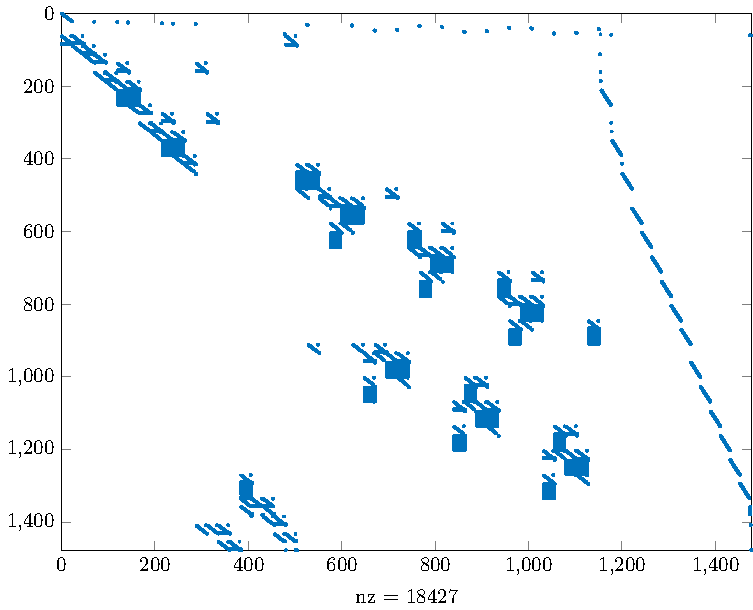
\includegraphics[scale=0.8]{../src/figure/lhr01.pdf}
\caption{Sparsity representation of the \texttt{lhr01} matrix.}
\label{fig:lhr01}
\end{figure}
Figure~\ref{fig:lhr01} shows the sparsity pattern of the \texttt{lhr01} light hydrocarbon recovery matrix. This matrix is real and not symmetric. From a complex point of view it again can be considered non-hermitian. However this matrix is a lot less symmetric then the circuit equations that have been explored earlier. The iterative methods implemented in the provided executable fail in this case givig the error message: \\
\texttt{ILU factorization failed on equation 21.} \\
In this case the Gaussian elimination process is unstable. %TODO WHY???
 The direct solver however is able to solve the problem in $0.009011 s$ using \texttt{7.365 MB}.



\subsection{ship003}

\subsection{Fault639}